Neste capítulo, apresentamos a criação de um grafo da rede social do Colab com base na fonte de dados disponibilizada pela empresa. O conjunto de dados consiste em uma lista de arestas, onde os nós representam os usuários e as arestas representam as conexões ou seguidores desses usuários. Utilizamos diversas técnicas de análise de redes, incluindo o agrupamento de Louvain, o agrupamento espectral e a centralidade de Eigenvector.

O agrupamento de Louvain é um algoritmo de detecção de comunidades que busca otimizar a modularidade, uma medida da densidade de conexões dentro das comunidades em comparação com as conexões entre as comunidades. Já o agrupamento espectral é uma técnica que utiliza os Eigenvectors do grafo para particionar os nós em comunidades. Além disso, exploramos a centralidade de Eigenvector para identificar os nós centrais na rede, ou seja, aqueles com maior influência ou importância. Essa medida utiliza os Eigenvectors para determinar a importância de um nó com base em sua conexão com outros nós na rede. Dessa forma, por meio dessas técnicas de análise de redes, buscamos compreender a estrutura e os padrões presentes na rede social do Colab.

Este estudo baseia-se em pesquisas anteriores que utilizaram a análise de redes para estudar redes sociais, como o Twitter e o Facebook, a fim de obter insights sobre a estrutura dessas comunidades. Por exemplo, \citeonline{2006_Newman} utilizaram o agrupamento espectral para identificar comunidades em uma rede de blogs políticos e mostraram que essas comunidades eram altamente polarizadas.

\subsection*{Pré-processamento do conjunto de dados Colab}
\label{sec:preprocessing}

Antes de carregar os dados em scripts e aplicações, realizamos algum pré-processamento nos arquivos CSV brutos usando a biblioteca Pandas do Python. O CSV original era uma lista de arestas em que a coluna "source" representava um usuário e a coluna "target" representava uma conexão com outro usuário. O arquivo CSV também tinha colunas para registrar quando essas relações foram criadas, atualizadas e excluídas, o que pode ser usado para adicionar dinâmica temporal à visualização. No entanto, os carimbos de data e hora originais estavam no formato brasileiro e precisaram ser convertidos para o formato ISO 8601, que é o padrão em SNA.

Outra etapa foi separar a tabela de arestas dos dados dos nós, dedicando um arquivo para as relações dos usuários expressas por meio das colunas "source" e "target", e outro arquivo para os dados dos nós dos usuários. Esses arquivos são edges.csv e nodes.csv, respectivamente. Neste momento, o arquivo de nós contém apenas dados temporais, mas mais adiante no experimento, pretendemos incorporar também dados de localização, por isso decidimos dividir os arquivos. Isso também é considerado um padrão mais consistente para carregar uma lista de arestas no em modelos baseados em grafos, conforme demonstrado por \citeonline{2016_Golbeck_PAGE}.

Também removemos nós duplicados. No contexto dos dados brutos, a coluna 'deleted\_at' representa quando um usuário foi deixado de seguir por outro usuário. Essa métrica nos fornece uma visão mais ampla do modelo de comunidade, mas, por simplicidade, optamos por removê-la deste primeiro experimento no Gephi. Retomaremos o estudo sobre a ação de deixar de seguir usuários posteriormente.

Para aproveitar o poder computacional, usamos o Google Colaboratory para realizar o pré-processamento dos dados. O script abaixo adapta as colunas de carimbos de data e hora e remove as linhas duplicadas.

\section{Construção de grafo da Rede Social}
A análise das interações dos usuários dentro do aplicativo Colab requer a criação de um grafo de rede social, a fim de representar visualmente as conexões entre os usuários e suas respectivas postagens. Dado que o banco de dados original do Colab é um banco de dados relacional, foi necessário realizar a transformação dos dados em uma estrutura de grafo.

A transformação dos dados de lista de arestas em uma estrutura de grafo permitiu uma representação mais adequada das relações e interações entre os usuários. Essa transformação envolveu a representação de cada usuário como um nó no grafo e a mapeamento das conexões entre os usuários como arestas.

Essa abordagem apresenta algumas vantagens importantes em relação à análise de redes sociais. Ao utilizar um formato de dados em grafo, foi possível visualizar e analisar a estrutura da rede de forma mais intuitiva, identificando grupos de usuários e suas interações com maior clareza. Além disso, a representação em grafo facilita a aplicação de algoritmos de análise de redes, como algoritmos de agrupamento e detecção de comunidades, que podem revelar informações relevantes sobre a estrutura da rede e a formação de câmaras de eco.

Essa estrutura de dados é obtida inicialmente no formato CSV, importada para o Gephi e eventualmente foi criado uma base de dados utilizando o Neo4j. Embora o Neo4j seja um exemplo de sistema de gerenciamento de banco de dados de grafos, é importante destacar que a transformação dos dados de um banco de dados relacional em um formato de grafo não está necessariamente vinculada a um sistema de gerenciamento de banco de dados específico. Existem várias ferramentas e bibliotecas disponíveis, como o NetworkX, que permitem a transformação de dados relacionais em estruturas de grafos para análise.

Portanto, ao realizar a transformação dos dados de um banco de dados relacional em uma estrutura de grafo, foi possível obter uma representação mais adequada das interações dos usuários no aplicativo Colab, permitindo uma análise mais detalhada e precisa da rede social. Essa abordagem oferece vantagens significativas na compreensão dos padrões de engajamento dos usuários e na identificação de câmaras de eco.

\subsection*{Introdução ao Gephi}

A análise exploratória de redes sociais (ESNA) é um passo fundamental para compreender as estruturas complexas e dinâmicas das redes sociais. Este trabalho é fundamentado na teoria dos grafos e os benefícios que essa abstração pode trazer para análise de redes sociais. Essa fundamentação é detalhada no \autoref{chapter:05_networkanalysis}. O primeiro passo na ESNA é visualizar os dados da rede, e o Gephi é uma das ferramentas mais populares e poderosas usadas nessa etapa. O Gephi é um software de análise e visualização de redes de código aberto que permite aos pesquisadores criar e manipular grafos, executar vários algoritmos de análise de rede e gerar representações visuais das estruturas de rede. O Gephi tem sido amplamente utilizado na análise de redes sociais (SNA) para analisar a estrutura e dinâmica dos relacionamentos sociais.

O Gephi possui muitos dos modelos e algoritmos mais comuns de SNA, como centralidade de grau, centralidade de intermediação e coeficiente de agrupamento. Essas medidas permitem que os pesquisadores examinem a importância de nós ou atores individuais dentro de uma rede, bem como a estrutura geral da rede. O software também inclui uma variedade de algoritmos de layout que permitem aos pesquisadores visualizar as estruturas de rede de diferentes maneiras, como o layout ForceAtlas2, que simula forças físicas entre os nós para criar uma representação visual clara da rede. O Gephi também pode ser usado para analisar a dinâmica temporal das redes sociais. Outra característica útil do Gephi é sua capacidade de lidar com conjuntos de dados grandes e complexos. O Gephi pode lidar com redes com milhões de nós e arestas, tornando-se uma ferramenta valiosa para analisar redes sociais em larga escala. Particularmente para este estudo, uma área em que o Gephi tem sido útil é na detecção de câmaras de eco em redes sociais. Por exemplo, em um estudo de \citeonline{2021_Conover}, o Gephi foi usado para analisar as conversas no Twitter em torno das eleições legislativas dos Estados Unidos em 2010, revelando a existência de comunidades ideologicamente segregadas.

Para detectar câmaras de eco usando o Gephi, os pesquisadores primeiro precisam coletar dados sobre a rede social de interesse. Isso pode ser feito usando uma variedade de métodos, como web scraping, chamadas de API ou pesquisas. Uma vez que os dados são coletados, eles podem ser importados para o Gephi e visualizados usando as ferramentas de visualização de rede do software. Pesquisadores podem então usar vários algoritmos de SNA para identificar os nós mais centrais dentro da rede, bem como as diferentes comunidades ou subgrupos dentro da rede. No caso dessa pesquisa, utilizamos os dados da \autoref{tab:connections_model}.

\begin{figure}[!htb]
	\caption{Importando dados no Gephi}
	\label{fig:gephi_edge_import}
	\centering
	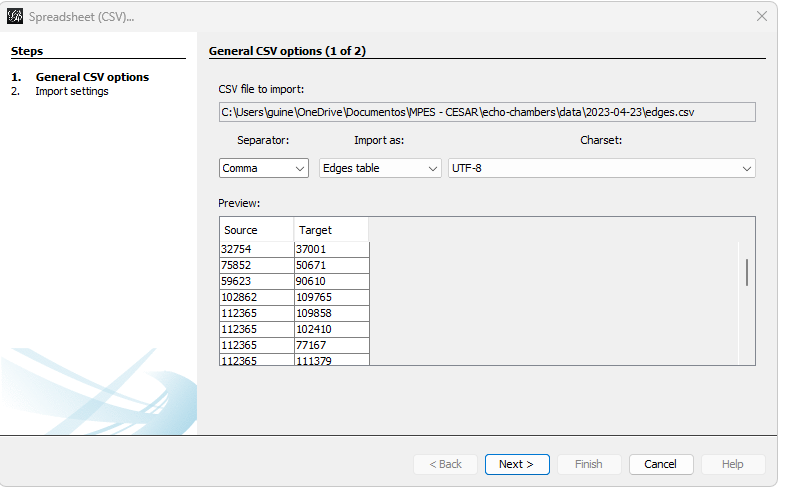
\includegraphics[scale=0.6]{images/gephi-edge-import.png}
\end{figure}

\subsection*{Carregando o conjunto de dados Colab no Gephi}
Após baixar o arquivo pré-processado descrito em \autoref{sec:preprocessing}, criamos um novo Workspace no Gephi e carregamos os arquivos de dados separadamente, começando pelo edges.csv. O arquivo nodes.csv é então carregado e o Gephi detecta automaticamente os carimbos de data e hora. Após importar ambos os arquivos, a tabela de dados do Gephi exibe os nós, as arestas e os carimbos de data e hora. A importação detectou 33818 nós e 66875 arestas. No entanto, devido ao alto número de conexões, a visualização do gráfico do Gephi exibe apenas um quadrado preto. Para corrigir isso e obter informações iniciais do conjunto de dados, precisamos escolher um Layout apropriado usando a guia de layout do Gephi.

\begin{figure}[!htb]
	\caption{Modelo de dados carregado no Gephi}
	\label{fig:gephi_data_table}
	\centering
	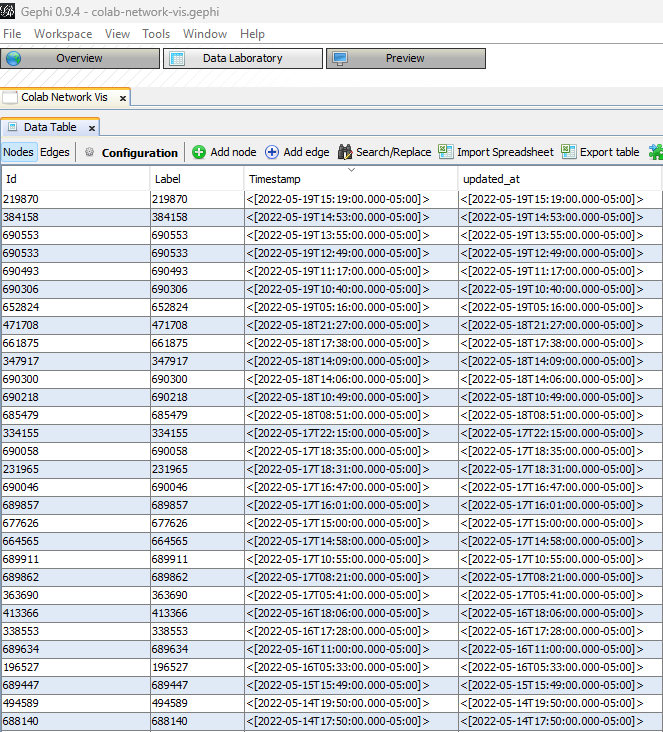
\includegraphics[scale=0.8]{images/gephi-data-table.png}
\end{figure}

\subsection*{Compreendendo os Layouts do Gephi}

Os layouts são um aspecto essencial da funcionalidade do Gephi, pois eles fornecem uma representação gráfica da estrutura da rede. O Gephi oferece vários presets de layout para gerar visualizações dos dados da rede em diversas formas. Cada preset utiliza um conjunto único de algoritmos para posicionar os nós e arestas da rede de maneira visualmente atraente. Nesta seção, examinaremos alguns dos layouts mais comuns do Gephi, seus casos de uso e sugeriremos o melhor layout para uma rede com tantas conexões.

Um dos layouts mais utilizados no Gephi é o layout Force Atlas. O layout Force Atlas é um layout baseado em forças que simula a física de um sistema massa-mola para organizar os nós da rede. Esse layout é particularmente útil para visualizar redes sociais, pois pode destacar aglomerados e comunidades de nós. O layout Force Atlas é especialmente adequado para redes de tamanho pequeno a médio, pois pode se tornar computacionalmente caro para redes maiores.

O layout Fruchterman-Reingold é outro layout popular no Gephi. Também é um layout baseado em forças que equilibra as forças de atração e repulsão entre os nós. Esse layout é particularmente útil para visualizar redes de tamanho pequeno a médio e pode ser usado para destacar aglomerados e comunidades de nós.

O layout Yifan Hu é um algoritmo baseado em forças desenvolvido por Yifan Hu em 2005. O algoritmo utiliza uma abordagem multinível para otimizar o layout dos nós em uma rede, minimizando uma função de energia que equilibra as forças de repulsão e atração entre os nós. Em cada nível, o algoritmo constrói uma representação mais grosseira da rede e a utiliza para guiar o layout da rede em níveis mais finos. Essa abordagem permite que o algoritmo lide com redes grandes e complexas, reduzindo a complexidade computacional do processo de layout. O layout Yifan Hu foi integrado em várias ferramentas de visualização de redes, incluindo o Gephi, como uma opção de layout padrão. A eficácia do layout foi demonstrada em diversos estudos, incluindo um estudo realizado por Lin (2019), que utilizaram o layout para visualizar a rede de coautoria de uma disciplina científica. Os resultados mostraram que o layout Yifan Hu foi capaz de visualizar efetivamente a estrutura da comunidade e destacar autores e publicações importantes dentro da rede.

Para uma rede com 66875 arestas, optamos por usar o layout Yifan Hu devido à sua capacidade de lidar com redes de grande escala, tornando-o adequado para o tamanho da rede fornecido. Além disso, o layout Yifan Hu é baseado em forças e pode otimizar o layout dos nós para fornecer uma representação visualmente agradável da rede. Posteriormente no experimento, pretendemos utilizar outros modelos de layout para obter diferentes insights do modelo de dados.

\subsection*{Visualizações do Gephi da Rede Colab}

O layout Yifan Hu foi aplicado ao conjunto de dados do Colab, resultando nesta imagem que apresenta dois clusters bem populados, uma quantidade considerável de nós de usuário e um grande número de nós isolados.

\begin{figure}[!hbtp]
	\caption{Rede do Colab renderizada com Layout Yifan Hu}
	\label{fig:colab_yifan_hu_first_set}
	\centering
	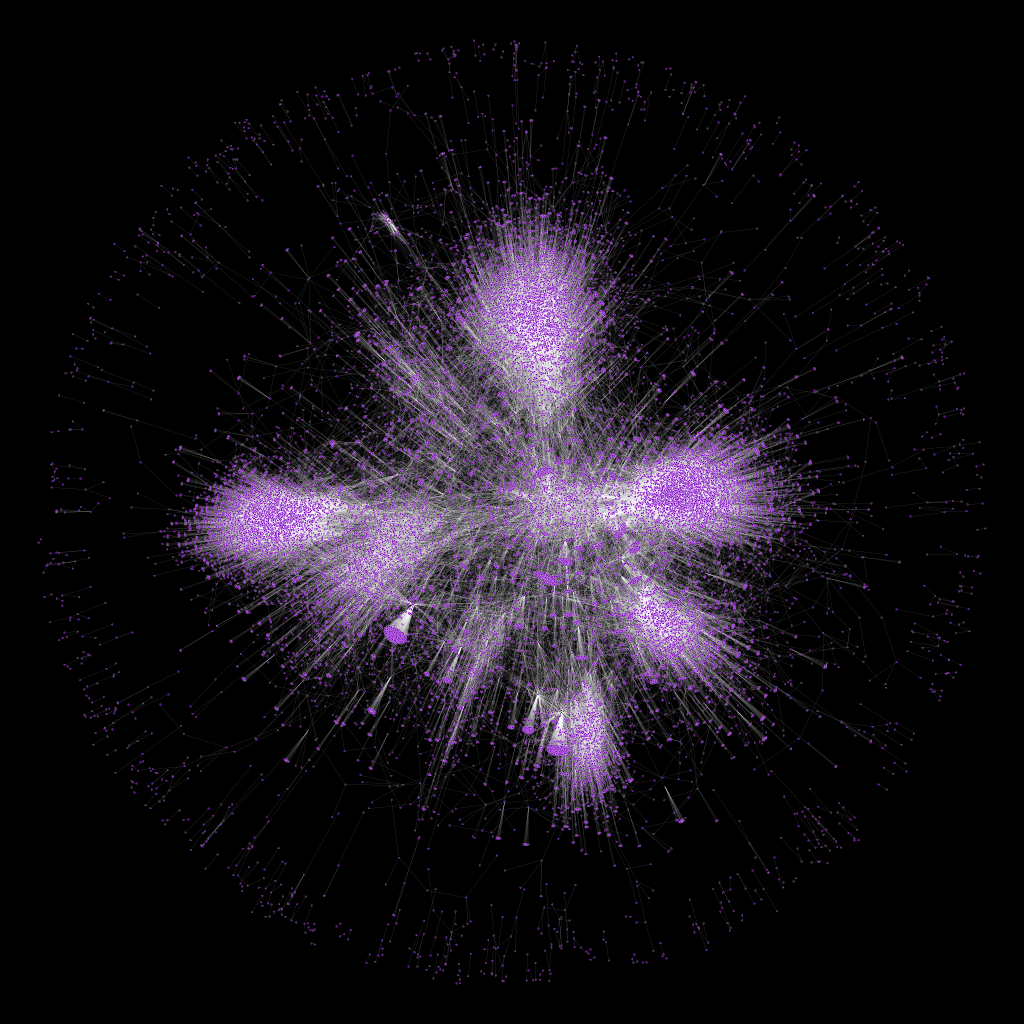
\includegraphics[scale=0.2]{images/colab-yifan-hu-first-set.png}
\end{figure}

O Yifan Hu nos proporciona um bom ponto de partida e algumas ideias iniciais. No entanto, para obter mais informações sobre o conjunto de dados, precisamos executar algumas estatísticas no Gephi e atualizar a aparência da visualização com os resultados das estatísticas. Vamos começar introduzindo as várias estatísticas do Gephi e avaliar como nossa análise de câmara de eco pode se beneficiar melhor de cada uma delas.

\subsection*{Explorando a Estrutura da Rede com as Estatísticas do Gephi}

\begin{figure}[!htb]
	\caption{Rede do Colab renderizada com Layout Yifan Hu e aparência dos nós enfatizando Centralidade.}
	\label{fig:colab_apperance_centrality}
	\centering
	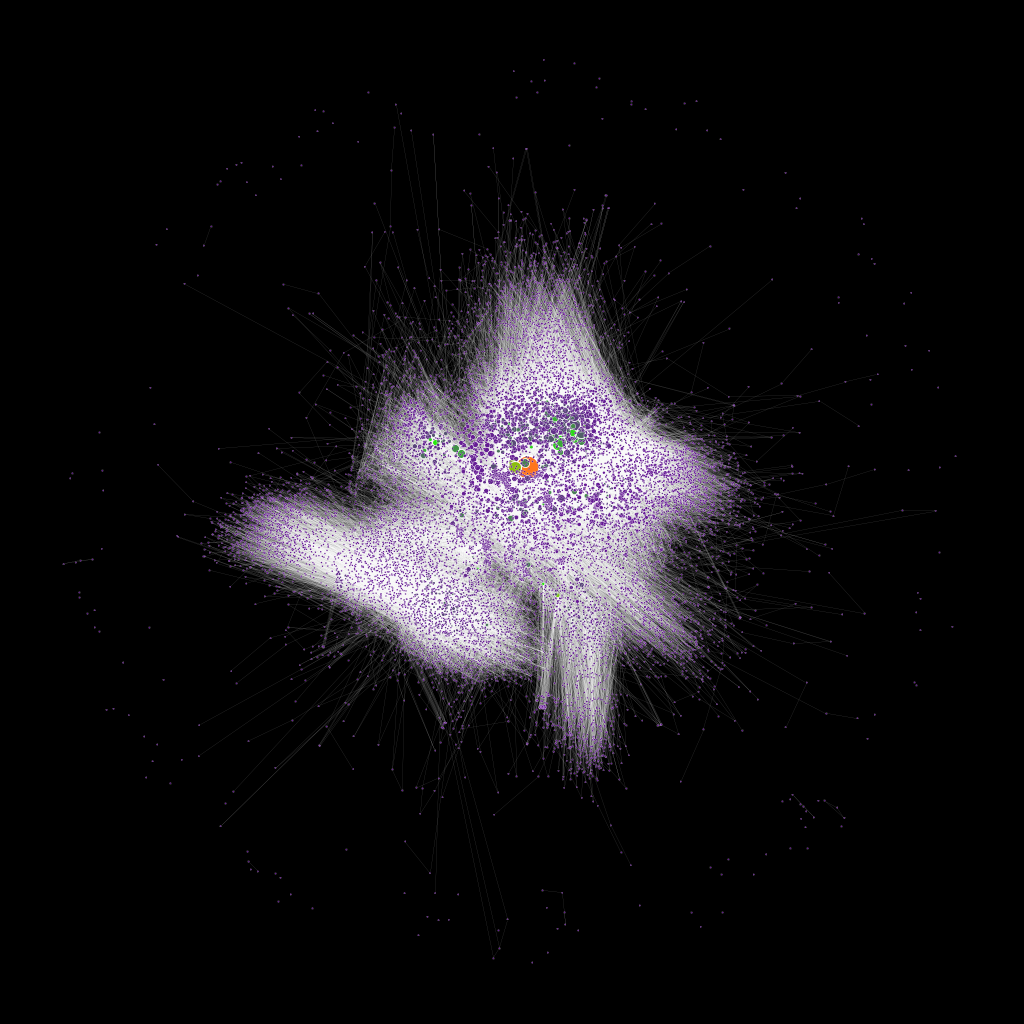
\includegraphics[scale=0.1]{images/colab-apperance-centrality.png}
	\fautor
\end{figure}

O Gephi oferece uma variedade de estatísticas que podem ajudar os pesquisadores a analisar e visualizar a estrutura das redes. Algumas das estatísticas mais comumente usadas na análise de redes sociais incluem grau, centralidade de intermediação (betweenness centrality) e coeficiente de agrupamento (clustering coefficient). O grau mede o número de conexões que um nó possui, enquanto a centralidade de intermediação identifica nós que desempenham um papel importante como pontes entre diferentes partes da rede. O coeficiente de agrupamento mede o grau em que os nós tendem a se agrupar em grupos.

Ao trabalhar com uma rede grande como o conjunto de dados do Colab, as estatísticas do Gephi podem ser particularmente úteis para obter insights sobre a estrutura subjacente da rede. Por exemplo, o grau pode ajudar a identificar nós com um grande número de conexões, enquanto a centralidade de intermediação pode destacar nós que são especialmente importantes para manter a conectividade geral da rede. O coeficiente de agrupamento pode ajudar a identificar grupos de nós que tendem a se agrupar, fornecendo informações sobre potenciais câmaras de eco ou outros padrões de agrupamento dentro da rede.

Algumas das estatísticas do Gephi mais úteis a serem consideradas incluem modularidade, detecção de comunidades e centralidade do Eigenvector. A modularidade mede o grau em que os nós dentro da rede se agrupam em grupos coesos, enquanto algoritmos de detecção de comunidades podem ajudar a identificar esses grupos com base em padrões de conectividade. A centralidade do Eigenvector, por outro lado, mede o grau em que um nó está conectado a outros nós altamente conectados dentro da rede.

Em nossa análise exploratória do conjunto de dados do Colab, começamos calculando o Diâmetro da Rede. A estatística de Diâmetro da Rede do Gephi mede a distância geodésica mais longa entre quaisquer dois nós na rede. Essa estatística é uma medida importante da conectividade da rede, pois reflete o grau em que os nós estão conectados entre si. Um diâmetro de rede baixo indica que os nós na rede estão intimamente conectados, enquanto um diâmetro de rede alto indica que os nós estão mais distantes uns dos outros. Essa estatística pode ser usada para identificar nós que são especialmente importantes para manter a conectividade da rede, bem como para detectar áreas da rede que podem estar mal conectadas.

A análise levou aproximadamente 10 minutos para ser concluída, o Diâmetro da Rede de 24 pode significar que a distância máxima entre quaisquer dois nós na rede é 24, indicando que a rede é relativamente compacta e bem conectada levando em conta o número total de nós. O Comprimento médio do caminho de 5.6 indica que, em média, são necessários pouco mais de cinco passos e meio para ir de um nó a outro na rede. Isso sugere que a rede possui caminhos relativamente curtos entre os nós, facilitando o fluxo de informações e influência pela rede. No geral, esses resultados sugerem que a rede está bem conectada, com um alto grau de interconectividade entre os nós.

Os resultados do Diâmetro da Rede e do comprimento médio do caminho sozinhos não são suficientes para determinar se a rede possui câmaras de eco. O diâmetro da rede e o comprimento médio do caminho fornecem informações sobre a estrutura geral da rede e como a informação pode se espalhar por ela. No entanto, para identificar câmaras de eco, precisamos examinar o coeficiente de agrupamento, a modularidade ou outras estatísticas de detecção de comunidades. Câmaras de eco geralmente têm níveis altos de agrupamento e uma pontuação baixa de modularidade, indicando grupos coesos que estão mais conectados entre si do que com o restante da rede. Ainda assim, podemos usar as configurações de aparência do Gephi para obter alguns insights adicionais. Depois de executar o algoritmo de diâmetro da rede, podemos usar suas métricas resultantes para alterar a aparência da nossa visualização da rede.

Especificamente, os nós foram coloridos de acordo com sua classificação de Centralidade de Proximidade (Closeness Centrality) e dimensionados de acordo com sua classificação de Centralidade de Intermediação (Betweenness Centrality). Essa abordagem permitiu uma representação clara dos nós que possuem alta centralidade em termos de sua importância na rede. Os nós com alta Centralidade de Proximidade foram coloridos em tons mais escuros de roxo, enquanto os nós com alta Centralidade de Intermediação foram dimensionados em tamanho maior. Essa combinação de atributos dos nós destacou efetivamente os nós mais importantes em termos de sua conectividade e posição na rede. Isso pode ajudar a identificar nós que são mais centrais para a rede, pois serão coloridos em tons mais escuros. Além disso, pode ajudar a identificar nós que estão mais isolados do restante da rede, pois serão coloridos em tons de laranja.

\subsection*{Otimizando visualizações com Filtragem no Gephi}

Em ambas as imagens, é perceptível uma prevalência de nós isolados. Após uma análise mais aprofundada, descobrimos que a maioria dos nós isolados são de fato de usuários sem seguidores no arquivo de conexões. Alguns deles são de usuários que seguiram outro usuário em algum momento, mas deixaram de seguir dentro do período em que o conjunto de dados foi capturado. Para mitigar a quantidade de nós isolados, utilizamos a filtragem do Gephi, pois ela pode ser aplicada apenas na visualização, preservando o conjunto de dados. A filtragem é uma etapa essencial na análise de redes, pois permite que os pesquisadores foquem em aspectos específicos da rede e removam informações irrelevantes ou ruidosas. No contexto da detecção de câmaras de eco, a filtragem é especialmente crucial, pois ajuda a identificar comunidades relevantes e reduz o impacto de nós isolados que podem não ser representativos da estrutura geral da rede. A filtragem é uma etapa crucial na análise de redes e tem sido amplamente estudada na literatura.
\citeonline{2016_Fortunato} destacaram a importância da filtragem na detecção de comunidades, pois ela pode impactar significativamente a qualidade e a precisão dos resultados. Da mesma forma, \citeonline{2010_Newman_BOOK} discutiu os desafios de lidar com dados ruidosos na análise de redes e sugeriu várias técnicas de filtragem para melhorar a qualidade da análise. Em particular, a filtragem com base no grau tem sido amplamente utilizada na análise de redes, pois permite que os pesquisadores foquem nos nós e comunidades mais importantes da rede \cite[]{2002_Borgatti}.

Para filtrar nós irrelevantes ou isolados, aplicamos várias etapas de filtragem no laboratório de dados do Gephi. Começamos removendo laços e arestas múltiplas, que podem criar informações redundantes e complicar a análise. Em seguida, removemos nós com baixo grau, ou seja, aqueles que possuíam poucas conexões com outros nós na rede. Optamos por usar um filtro de Grau a partir de 4 para destacar apenas comunidades compostas por pelo menos 4 usuários. Essa etapa nos permitiu focar em comunidades que tinham mais probabilidade de serem significativas em termos de fluxo de informações e interações de usuários. Também removemos nós que não estavam conectados a nenhum outro nó na rede.

\section{Topologia da Rede Colab}
Após aplicar as configurações de aparência, os agrupamentos de usuários se tornam mais visíveis, assim como a centralidade de alguns usuários-chave. No entanto, ainda existem outras estatísticas que podemos executar no Gephi para obter uma visão mais abrangente. A tabela abaixo apresenta um resumo de todas as métricas obtidas a partir das Estatísticas do Gephi:

\begin{table}[h]
	\centering
	\caption{Resumo das Estatísticas do Gephi}
	\label{tab:colab_gephi_statistics}
	\begin{tabular}{|l|l|l|}
		\hline
		\textbf{Relatório Gephi}    & \textbf{Chave}               & \textbf{Valor}     \\
		\hline
		Topologia                   & Nós                          & 33818              \\
		Topologia                   & Arestas                      & 66875              \\
		Diâmetro da Rede            & Comprimento Médio do Caminho & 5.623615966246081  \\
		Modularidade                & Modularidade                 & 0.683              \\
		Modularidade                & Número de Comunidades        & 352                \\
		Centralidade de Eigenvector & Mudança da Soma              & 0.3087450789952254 \\
		Centralidade de Eigenvector & Número de Iterações          & 100                \\
		Coeficiente de Agrupamento  & Média                        & 0.171              \\
		Componentes Conectados      & Fracamente Conectados        & 329                \\
		Componentes Conectados      & Fortemente Conectados        & 28119              \\
		PageRank                    & Epsilon                      & 0.001              \\
		PageRank                    & Probabilidade                & 0.85               \\
		Inferência Estatística      & Comprimento da Descrição     & 1184001.357        \\
		Inferência Estatística      & Número de Comunidades        & 1367               \\
		\hline
	\end{tabular}
\end{table}

Os resultados das estatísticas do Gephi executadas no conjunto de dados do Colab fornecem informações sobre a estrutura da rede e as potenciais câmaras de eco. O diâmetro da rede de 24 e o comprimento médio do caminho de 5,62 indicam que a rede é relativamente pequena e fortemente conectada. Isso sugere que as informações podem se espalhar rapidamente pela rede e que pode haver um alto grau de homofilia entre os nós, o que pode contribuir para a formação de câmaras de eco \cite[]{2012_Kadushin_BOOK}.

O valor de modularidade de 0,683 e o número de comunidades de 352 sugerem que a rede possui um grau relativamente alto de estrutura de comunidades, com muitos grupos distintos de nós que estão mais densamente conectados entre si do que a nós fora de sua comunidade. Isso é consistente com a ideia de câmaras de eco, já que grupos mais densamente conectados e insulares podem ser mais propensos a desenvolver e reforçar crenças e valores compartilhados \cite[]{2016_Vicario}.

Os valores de centralidade de eigenvector, com mudança total de 0,31 e número de iterações de 100, sugerem que existem alguns nós altamente influentes na rede que têm um impacto desproporcional na propagação de informações. Isso está de acordo com a ideia de "líderes de opinião" ou "influenciadores" em redes sociais
\cite[]{1955_Katz_BOOK}. Esses nós podem desempenhar um papel fundamental na formação e no reforço de câmaras de eco, já que suas crenças e valores podem ter mais probabilidade de se espalhar pela rede.

O coeficiente de clusterização médio de 0,171 sugere que existe um grau moderado de agrupamento na rede, ou seja, os nós tendem a se conectar a outros nós que já estão conectados a eles. Isso pode contribuir para a formação de câmaras de eco, já que nós que compartilham crenças ou valores têm mais probabilidade de se agrupar juntos \cite[]{1998_Watts}.

Os valores de componentes conectados, com 329 fracamente conectados e 28.119 fortemente conectados, sugerem que a rede possui um grande número de componentes fortemente conectados, ou seja, existem muitos grupos de nós que estão completamente ou quase completamente conectados entre si, mas não a outros nós na rede. Isso está de acordo com a ideia de câmaras de eco, já que grupos mais fortemente conectados e insulares podem ser mais propensos a desenvolver crenças e valores compartilhados \cite[]{2016_Vicario}.

Os valores de PageRank, com epsilon de 0,001 e probabilidade de 0,85, sugerem que existem alguns nós altamente influentes na rede que têm um impacto significativo na propagação de informações. Isso está em consonância com os resultados da centralidade de eigenvector e sugere que esses nós podem desempenhar um papel fundamental na formação e no reforço de câmaras de eco.

Os valores de inferência estatística, com comprimento da descrição de 1.184.001,36 e número de comunidades de 1.367, sugerem que existem muitas comunidades distintas na rede com diferentes padrões de conexões e interações. Isso está de acordo com as estratégias de fornecimento de conteúdo do aplicativo, pois essas comunidades podem ser locais por natureza. Além disso, é consistente com os resultados de modularidade e sugere que pode haver múltiplas câmaras de eco dentro da rede com diferentes crenças e valores, embora não possamos afirmar isso com certeza sem levar em conta o aspecto de localização.

No geral, as estatísticas do Gephi fornecem evidências de que a rede possui um alto grau de estrutura de comunidades, agrupamento e nós influentes, o que pode contribuir para a formação e o reforço de câmaras de eco. No entanto, mais pesquisas são necessárias para confirmar se as câmaras de eco estão presentes na rede e como estão estruturadas.

\subsection{Centralizade de Rede}

\begin{figure}[!hbtp]
	\caption{Rede do Colab renderizada com Layout OpenOrd}
	\label{fig:colab_openord}
	\centering
	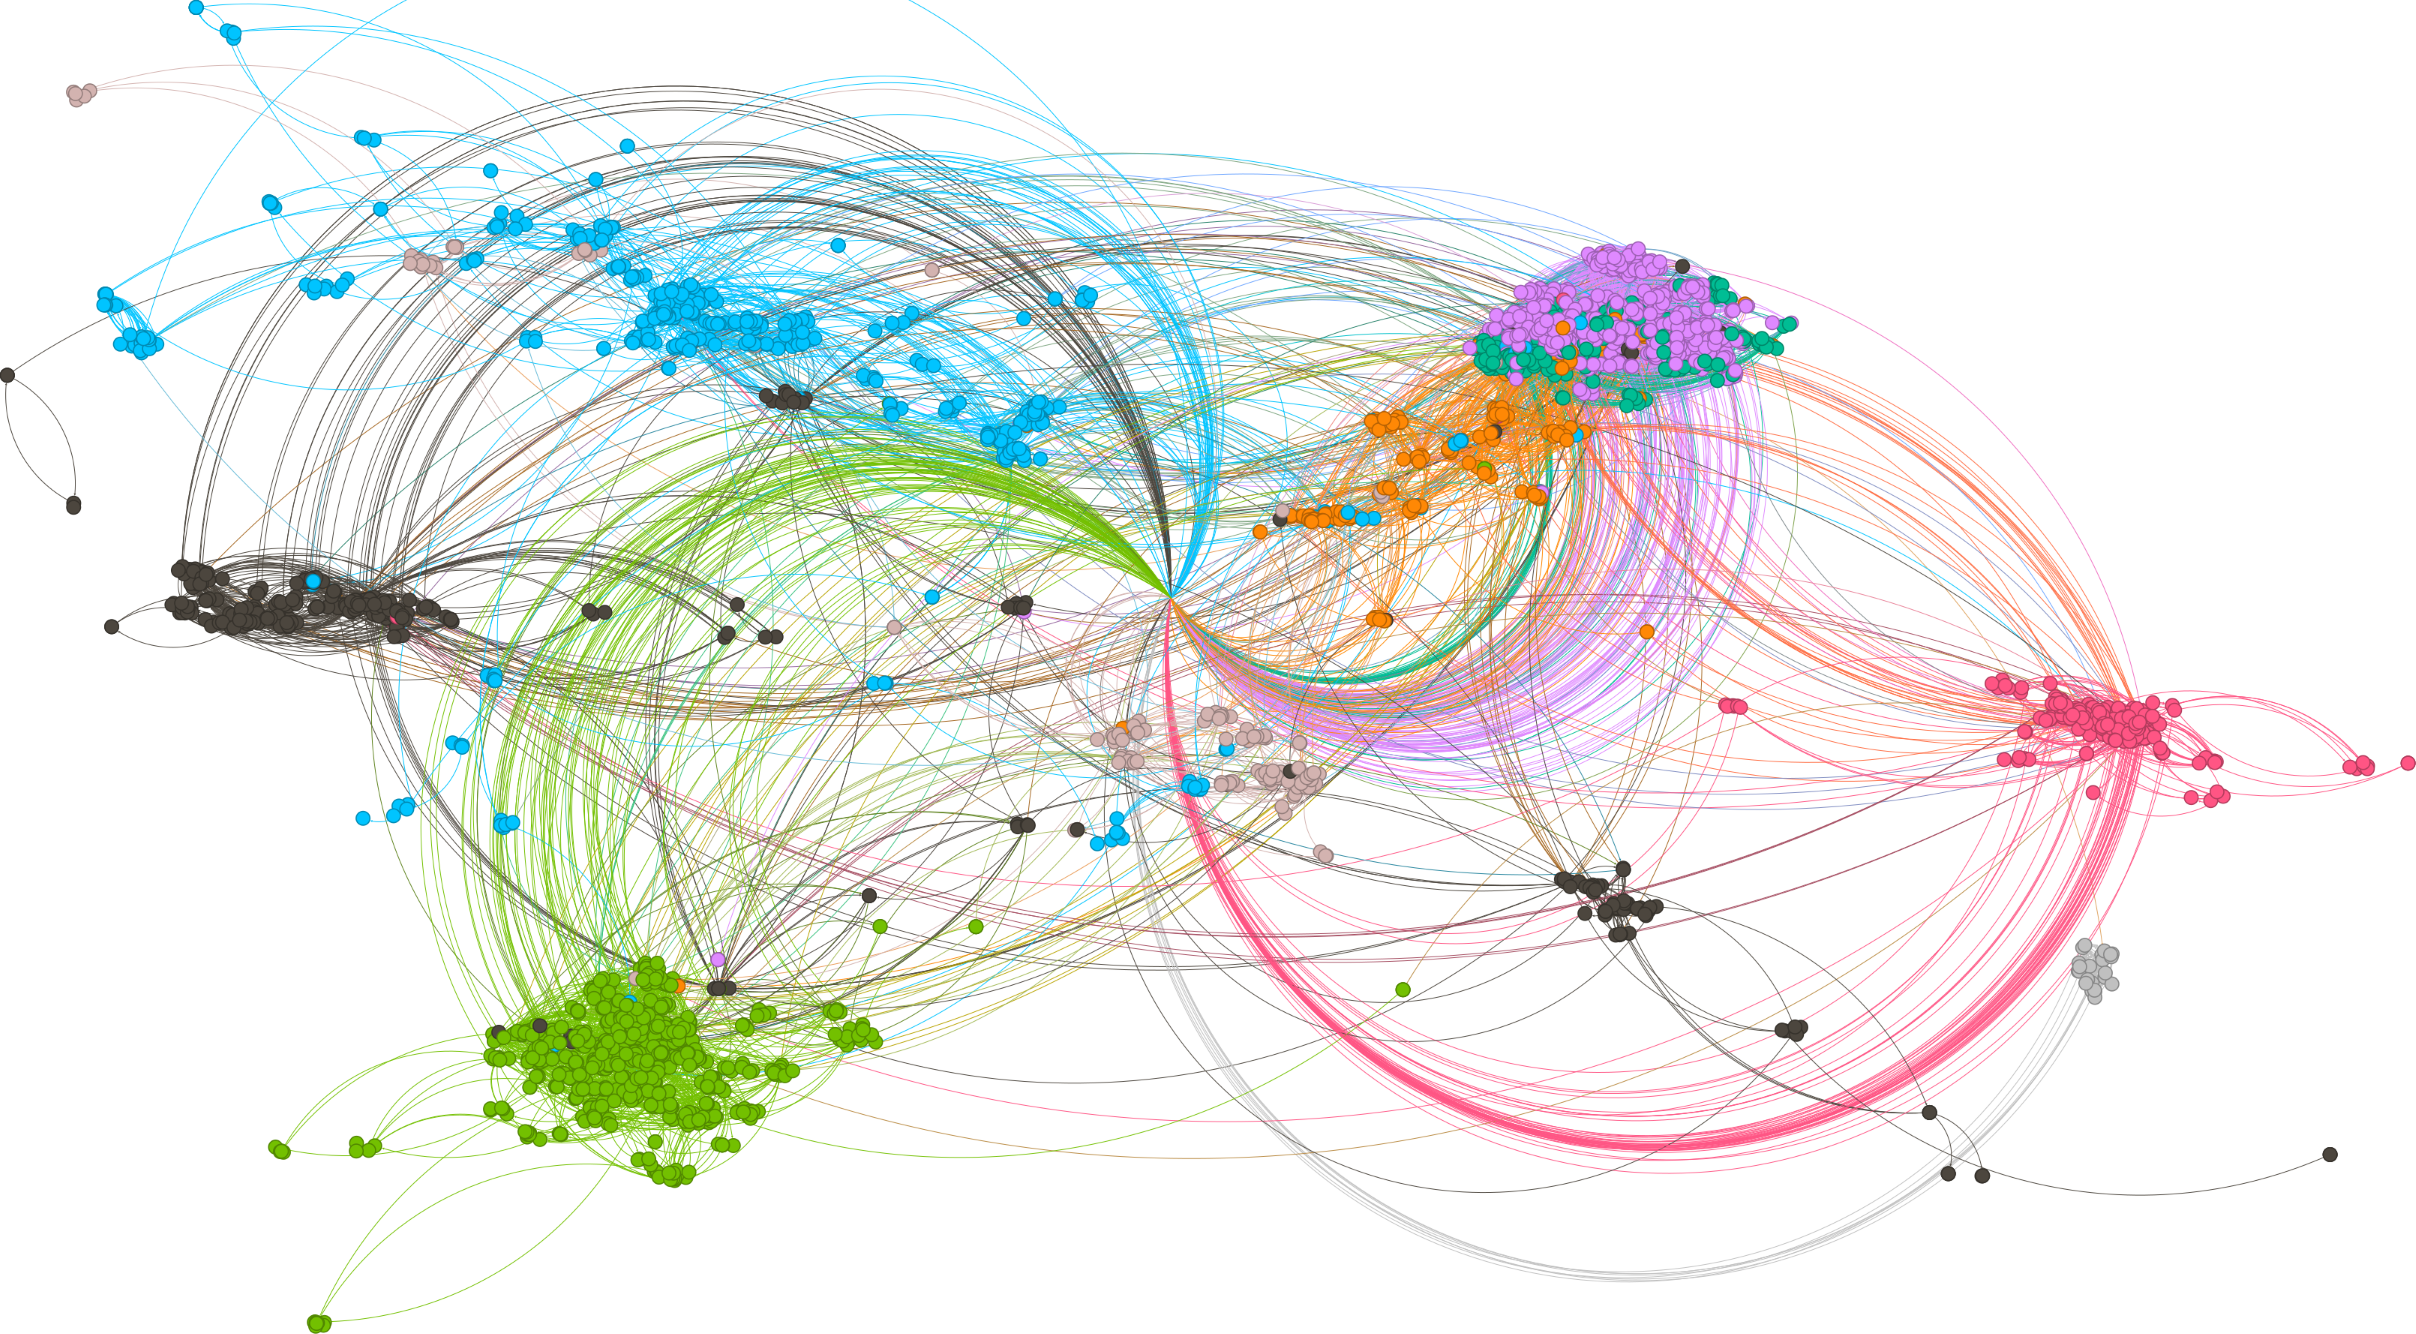
\includegraphics[scale=0.20]{images/colab-openord.png}
	\fautor
\end{figure}

Outra opção para visualizar centralidade é usar o algoritmo OpenOrd, um algoritmo de layout baseado em forças que é frequentemente usado em visualização e análise de redes. Uma das vantagens do algoritmo OpenOrd é sua capacidade de visualizar efetivamente a centralidade de intermediação em redes grandes e complexas. A centralidade de intermediação é uma medida da importância de um nó em uma rede, com base em sua capacidade de atuar como uma "ponte" ou "hub" entre diferentes partes da rede. Ao visualizar a centralidade de intermediação com o algoritmo OpenOrd, podemos identificar nós que desempenham um papel crucial na conexão de diferentes comunidades ou grupos dentro de uma rede.

Por exemplo, em um estudo sobre a comunicação no Twitter durante uma crise política, o algoritmo OpenOrd foi usado para visualizar a centralidade de intermediação de diferentes usuários do Twitter. Os resultados revelaram vários usuários com alta centralidade de intermediação, sugerindo que esses usuários desempenharam um papel fundamental na conexão de diferentes grupos de usuários do Twitter e na disseminação de informações durante a crise \cite[text]{2011_Poblete_IP}.

\begin{figure}[!hbtp]
	\caption{Rede do Colab destacando centralidade}
	\label{fig:colab_centrality}
	\centering
	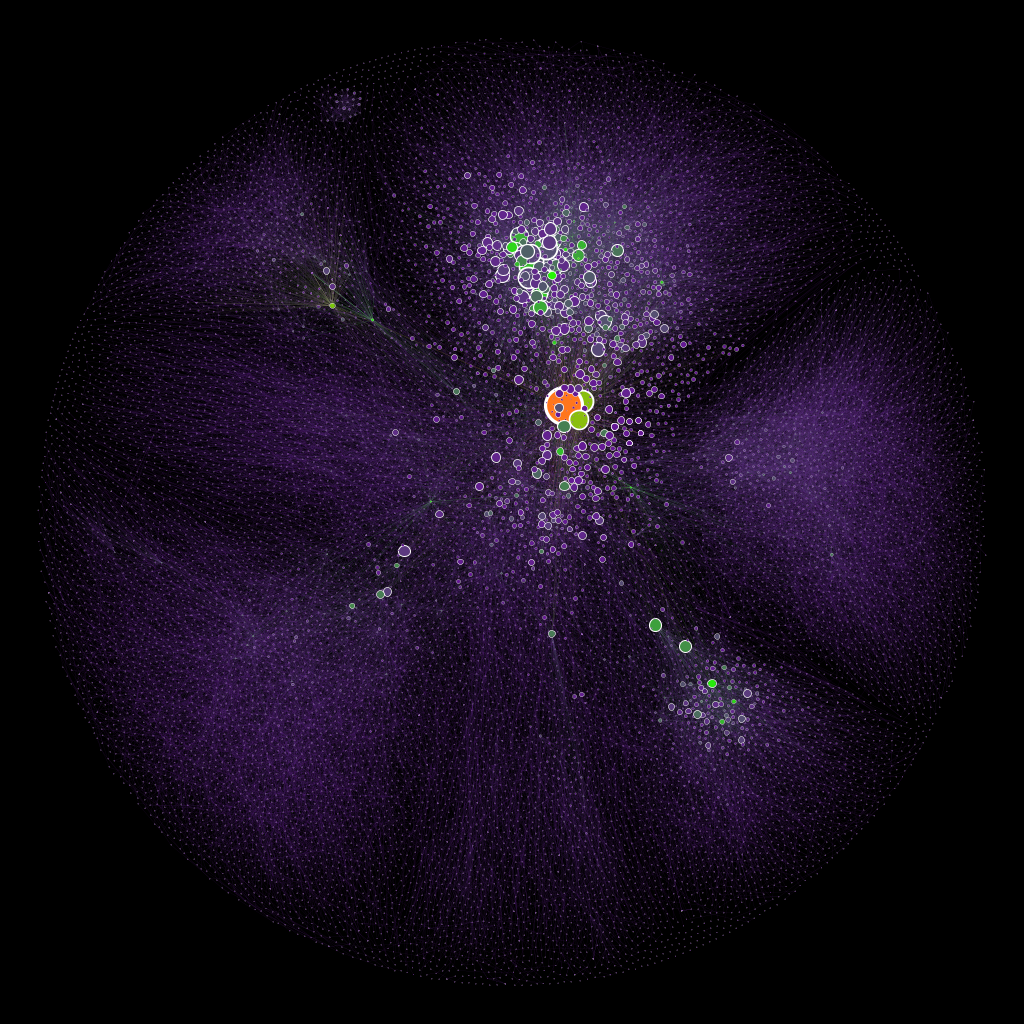
\includegraphics[scale=0.15]{images/colab-centrality.png}
	\fautor
\end{figure}

A visualização da rede Colab usando o algoritmo OpenOrd mostra uma clara distinção entre os nós com base em suas medidas de centralidade. Os nós maiores com maior centralidade de Eigenvector são mais influentes na rede e podem ter um impacto maior no fluxo de informações. O nó laranja, com a maior pontuação de centralidade de Eigenvector de 1.0, se destaca como o nó mais influente. No entanto, é interessante observar que esse nó tem uma pontuação de centralidade de intermediação relativamente baixa de 0.014, indicando que ele pode não servir necessariamente como um conector crítico entre diferentes partes da rede. Por outro lado, o nó verde no topo possui a segunda maior pontuação de centralidade de Eigenvector de 0.599 e pode atuar como um conector mais importante, com uma pontuação de centralidade de intermediação mais alta. No geral, os resultados sugerem que a rede é dominada por alguns nós altamente conectados, que podem ter um impacto significativo na estrutura e função geral da rede.

A centralidade desses usuários traz à tona o uso de cliques no contexto da Análise de Redes Sociais. Cliques podem ser um fator importante na identificação de câmaras de eco em redes. Um clique é um grupo de nós que estão todos conectados entre si, formando um subgrafo completo. Ao identificar cliques em uma rede, podemos começar a entender a estrutura da câmara de eco e como ela está conectada à rede mais ampla.

Para visualizar cliques no Gephi, uma abordagem é usar a estatística interna "Coeficiente de Agrupamento" para identificar nós que pertencem a aglomerados altamente conectados, que podem representar cliques. Após calcular o coeficiente de agrupamento para cada nó, é possível filtrar a rede para mostrar apenas nós com um coeficiente alto, como aqueles acima de um determinado limite. Em seguida, ajustando o tamanho e a cor dos nós na guia Aparência para refletir o número de conexões ou alguma outra métrica de interesse, os cliques podem ser visualizados como aglomerados densamente conectados de nós de cores e tamanhos semelhantes. Além disso, o uso dos algoritmos de agrupamento incorporados do Gephi, como o método Louvain ou otimização de modularidade, também pode ajudar a identificar e visualizar cliques em uma rede.

\begin{figure}[!hbtp]
	\centering
	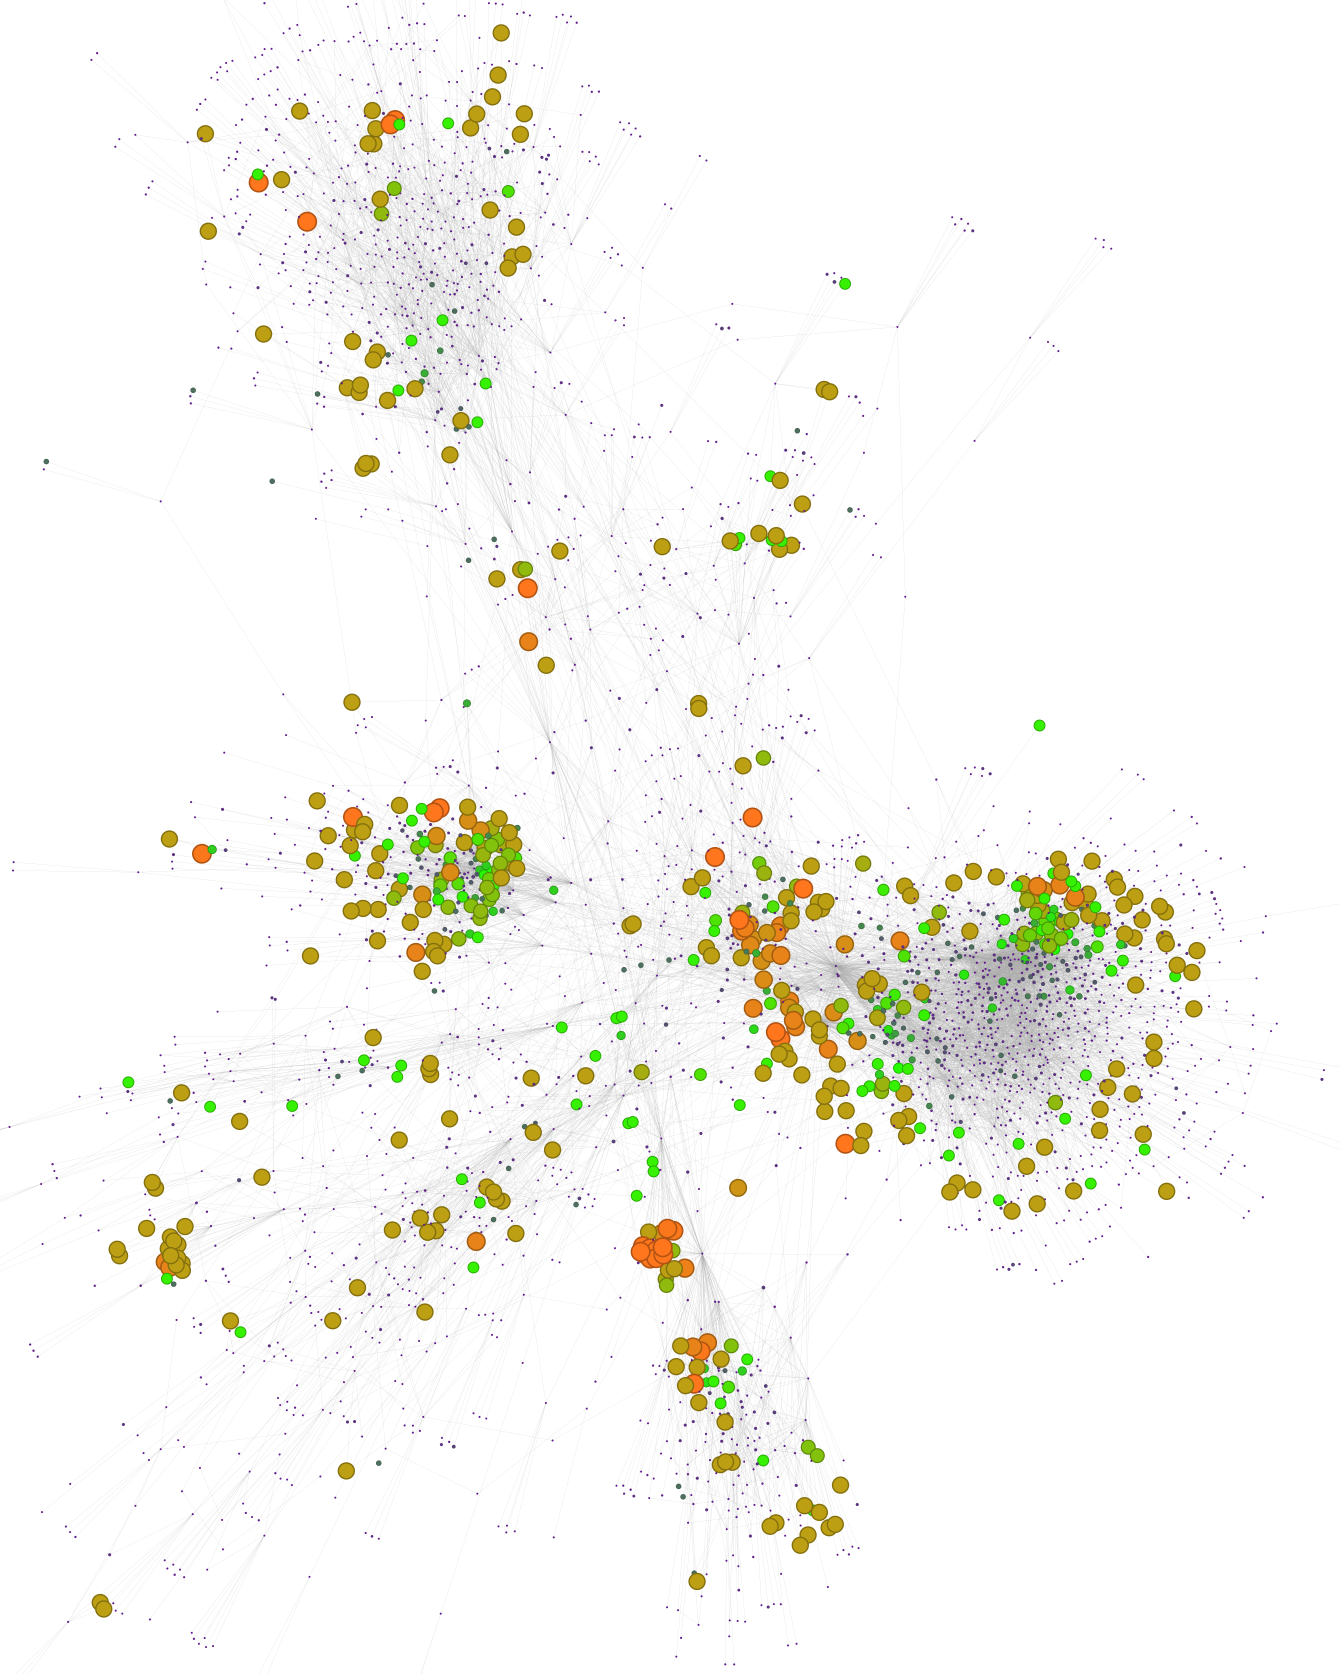
\includegraphics[scale=0.45]{images/colab-cliques.png}
	\caption{Visualização dos cliques identificados na rede. Nós que fazem parte de cliques são destacados em laranja, indicando subcomunidades altamente interconectadas. Nós verdes fazem parte de subcomunidades menores que orbitam os cliques. Nós roxos não fazem parte de nenhum clique.}
	\label{fig:gephi_cliques}
	\fautor
\end{figure}

Os cliques, sendo subgrafos completos, representam grupos de nós que estão altamente conectados entre si. Essa coesividade pode indicar subcomunidades fortemente interconectadas ou grupos de indivíduos com interações muito frequentes. A identificação desses cliques pode fornecer insights valiosos sobre a estrutura e dinâmica da rede, especialmente em contextos onde a formação de subgrupos coesos é de interesse, como em redes sociais ou colaborativas.

No entanto, apenas os cliques podem não ser suficientes para identificar câmaras de eco, pois podem estar em jogo outros fatores, como homofilia ou viés de confirmação. Portanto, é importante usar múltiplas abordagens e métricas, como detecção de comunidades e análise de conteúdo, para obter uma compreensão mais abrangente das câmaras de eco na rede.

Enquanto os cliques nos oferecem uma visão sobre subgrupos coesos dentro da rede, é essencial também considerar a influência individual de cada nó para compreender a dinâmica da rede como um todo. Nesse contexto, a centralidade de eigenvector emerge como uma métrica valiosa. Proposta por \citeonline{1972_Bonacich}, essa métrica não se limita a contar as conexões diretas de um nó, mas pondera essas conexões com base na influência dos nós a que estão conectadas. Assim, um nó conectado a outros nós influentes terá uma pontuação de centralidade de eigenvector mais alta. Esta métrica é particularmente útil para identificar atores-chave em redes sociais, pois destaca aqueles que, mesmo que não estejam diretamente conectados a muitos outros, estão estrategicamente posicionados na rede. Em nossa análise, a centralidade de eigenvector nos ajudará a identificar os usuários mais influentes no Colab, complementando nossa compreensão obtida através da identificação de cliques.

\begin{figure}[!hbtp]
	\caption{Visualização destacando os usuários mais influentes na rede}
	\label{fig:colab_users_graph}
	\centering
	\includegraphics[scale=0.28]{images/colab-users-graph.png}
	\fautor
\end{figure}

Na Figura \ref{fig:colab_users_graph}, a estatística de modularidade do Gephi foi empregada para discernir e colorir distintas comunidades na rede do Colab. Ao analisar a distribuição das comunidades, observa-se que as dez primeiras comunidades representam uma proporção significativa da rede, indicando que uma parte considerável dos nós está concentrada nessas comunidades principais.

A centralidade de eigenvector revela insights interessantes sobre a influência dos nós dentro dessas comunidades. Uma proporção notável de nós tem uma pontuação de eigenvector de 0,0, sugerindo que muitos usuários, embora pertencentes a comunidades, podem não ter uma influência direta significativa. No entanto, a presença de nós com pontuações de centralidade de eigenvector consideravelmente altas, até mesmo superiores a 1, destaca a existência de usuários-chave que atuam como hubs centrais em suas respectivas comunidades.

Estes hubs, com alta centralidade de eigenvector, desempenham um papel crucial na disseminação de informações e na formação de opiniões dentro de suas comunidades. Em algumas comunidades, observa-se mais de um hub, indicando uma estrutura de rede mais complexa com múltiplos canais de influência. Esta configuração sugere que, enquanto algumas comunidades podem ter um único ponto focal dominante, outras podem ter uma distribuição de influência mais equilibrada entre vários membros-chave.

A análise reforça a ideia de homofilia, onde usuários com opiniões ou características semelhantes tendem a se agrupar. A interação entre a estrutura das comunidades e a distribuição da centralidade de eigenvector sugere uma rede onde determinados usuários desempenham papéis cruciais, não apenas em termos de número de conexões, mas também em termos de influência qualitativa dentro de suas comunidades.

\subsection{Comunidades}

Visualizar um conjunto de dados do Gephi focando nas comunidades pode ser altamente benéfico para explorar a estrutura de redes complexas, como redes sociais, e identificar potenciais câmaras de eco. Ao identificar comunidades ou grupos dentro de uma rede, podemos obter insights sobre o comportamento de subgrupos dentro da rede maior e como eles podem interagir entre si. Uma abordagem popular para detectar comunidades em redes é o algoritmo de detecção de comunidades baseado em modularidade desenvolvido por \citeonline{2008_Blondel}. Esse algoritmo particiona os nós em comunidades, maximizando uma função de qualidade conhecida como modularidade, que mede a densidade de conexões dentro de uma comunidade em comparação com as conexões entre comunidades. Este método é frequentemente referido como o algoritmo "Louvain" em homenagem a instituição dos pesquisadores.

\subsection{Visualizando Comunidades no Gephi}

Ao configurar a aparência da visualização do Gephi, focamos em destacar as comunidades por meio de codificação de cores e tamanho. Especificamente, usamos a estatística de Modularidade para atribuir uma cor única a cada comunidade, facilitando a distinção visual entre diferentes subgrupos na rede. Além disso, aumentamos o tamanho dos nós dentro de cada comunidade para destacar sua importância dentro do subgrupo. Essas indicações visuais podem ajudar a identificar rapidamente potenciais câmaras de eco dentro da rede.

\begin{figure}[!hbtp]
	\caption{Rede do Colab destacando comunidades}
	\label{fig:colab_communities}
	\centering
	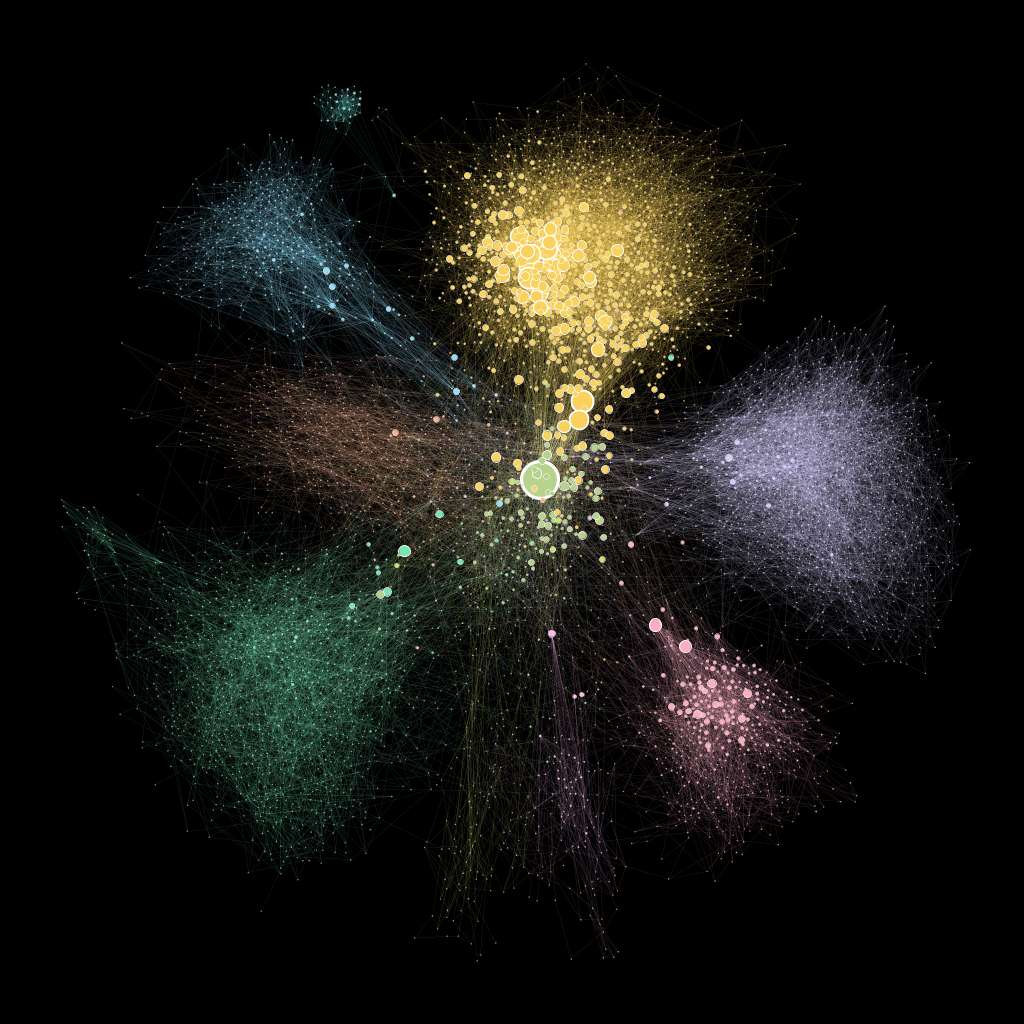
\includegraphics[scale=0.25]{images/colab-communities.png}
	\fautor
\end{figure}

Pesquisas mostram que visualizar comunidades dentro de uma rede pode ajudar a identificar câmaras de eco. Por exemplo, um estudo realizado por \citeonline{2018_Fortunato_IP} demonstrou que visualizar comunidades dentro de uma rede pode ajudar a detectar câmaras de eco e entender sua estrutura. Em nosso estudo, aplicamos abordagens semelhantes para detectar comunidades e visualizar nossa rede, o que nos permitiu identificar potenciais câmaras de eco e analisar ainda mais sua influência na disseminação de informações. O trabalho de \cite{2014_Colleoni} também 

Em resumo, visualizar um conjunto de dados do Gephi focando em comunidades pode fornecer insights valiosos sobre a estrutura de redes complexas e auxiliar na detecção de potenciais câmaras de eco. Ao usar codificação de cores e tamanho para destacar comunidades, podemos identificar rapidamente subgrupos dentro da rede e compreender melhor como eles interagem entre si. Essa abordagem é apoiada pelo trabalho de \citeonline{2010_Fortunato} e pode ser usada para obter insights sobre o comportamento de redes sociais e possíveis fontes de polarização.

\begin{figure}[!hbtp]
	\caption{Distribuição geográfica das comunidades da rede do Colab sobreposto ao mapa do Brasil}
	\label{fig:colab_geoclusters}
	\centering
	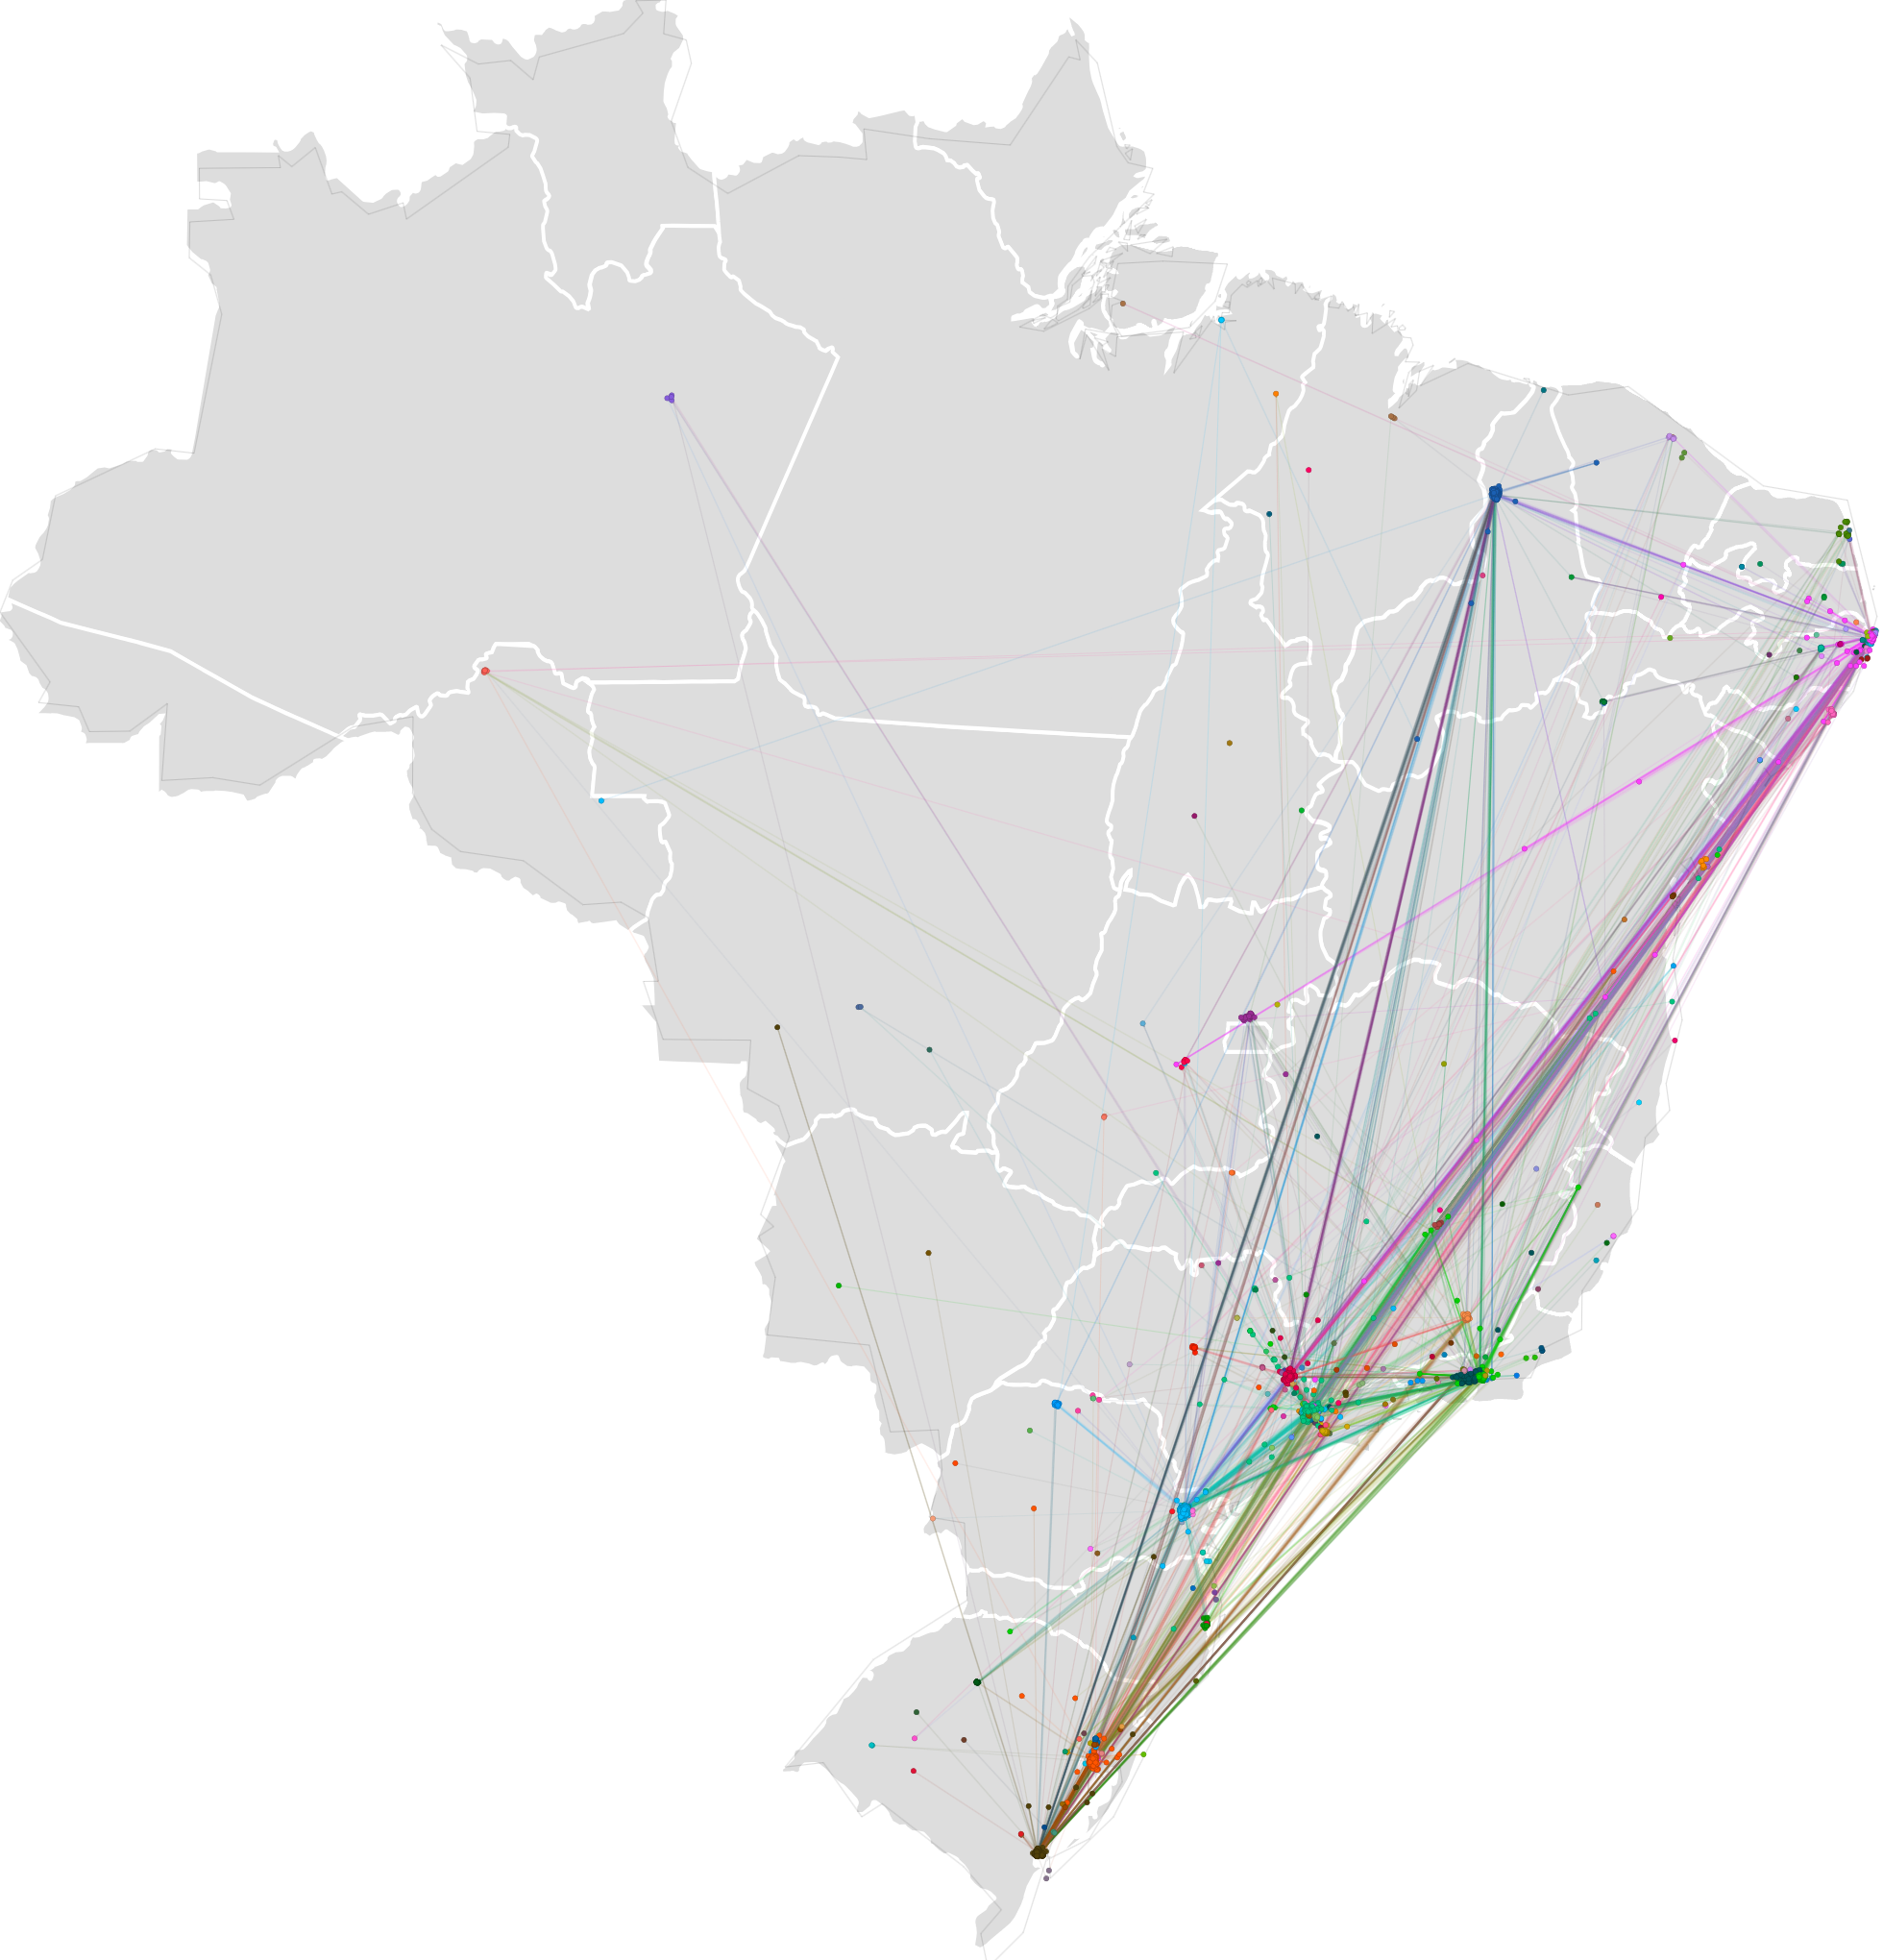
\includegraphics[scale=0.2]{images/colab-geocluster.png}
	\fautor
\end{figure}

A Figura \ref{fig:colab_geoclusters} apresenta a rede do Colab sobreposta a um mapa do Brasil, utilizando o GeoLayout do Gephi. Cada nó é colorido de acordo com o agrupamento de Louvain, e é notável que nós geograficamente próximos tendem a pertencer ao mesmo cluster. Isso sugere uma forte relação entre proximidade geográfica e formação de comunidades, reforçando o conceito de homofilia. Esta visualização também destaca as principais concentrações urbanas, permitindo uma análise mais aprofundada das dinâmicas sociais e potenciais câmaras de eco em diferentes regiões do país.

Ao nos aprofundarmos na análise da rede Colab, decidimos focar em um subset específico: os usuários das cidades de Mesquita, Niterói e Santo André. Esta granularização permite uma análise mais detalhada e contextualizada, levando em consideração as particularidades e dinâmicas sociais de cada cidade. Ao limitar nossa análise a essas cidades, podemos identificar padrões de conexão e interação que podem ser distintos em comparação com a rede geral. Esta abordagem focada aumenta a precisão na identificação de câmaras de eco, pois permite observar nuances e tendências que podem ser diluídas em uma análise de toda a rede. Além disso, ao entender as dinâmicas de câmaras de eco em níveis locais, podemos obter insights sobre como informações, crenças e valores são compartilhados e reforçados dentro de comunidades específicas, fornecendo uma base sólida para intervenções e estratégias direcionadas.

\section{Niterói, Santo André e Mesquita}

Prosseguindo com nossa investigação, decidimos concentrar nossos esforços nas cidades que apresentaram maior volume de interações no Colab. Assim, Niterói, Santo André e Mesquita emergem como os principais focos de nossa análise subsequente. Esta escolha não é aleatória, mas sim baseada na relevância e densidade de atividades nestas localidades. Ao nos concentrarmos nestas cidades, buscamos entender de forma mais precisa as dinâmicas e particularidades das interações e, consequentemente, das potenciais câmaras de eco que se formam nestes contextos específicos.

\begin{figure}[!htb]
	\caption{Rede do Colab destacando as cidades de Niterói, Santo André e Mesquita}
	\label{fig:colab_graph_3_cidades}
	\centering
	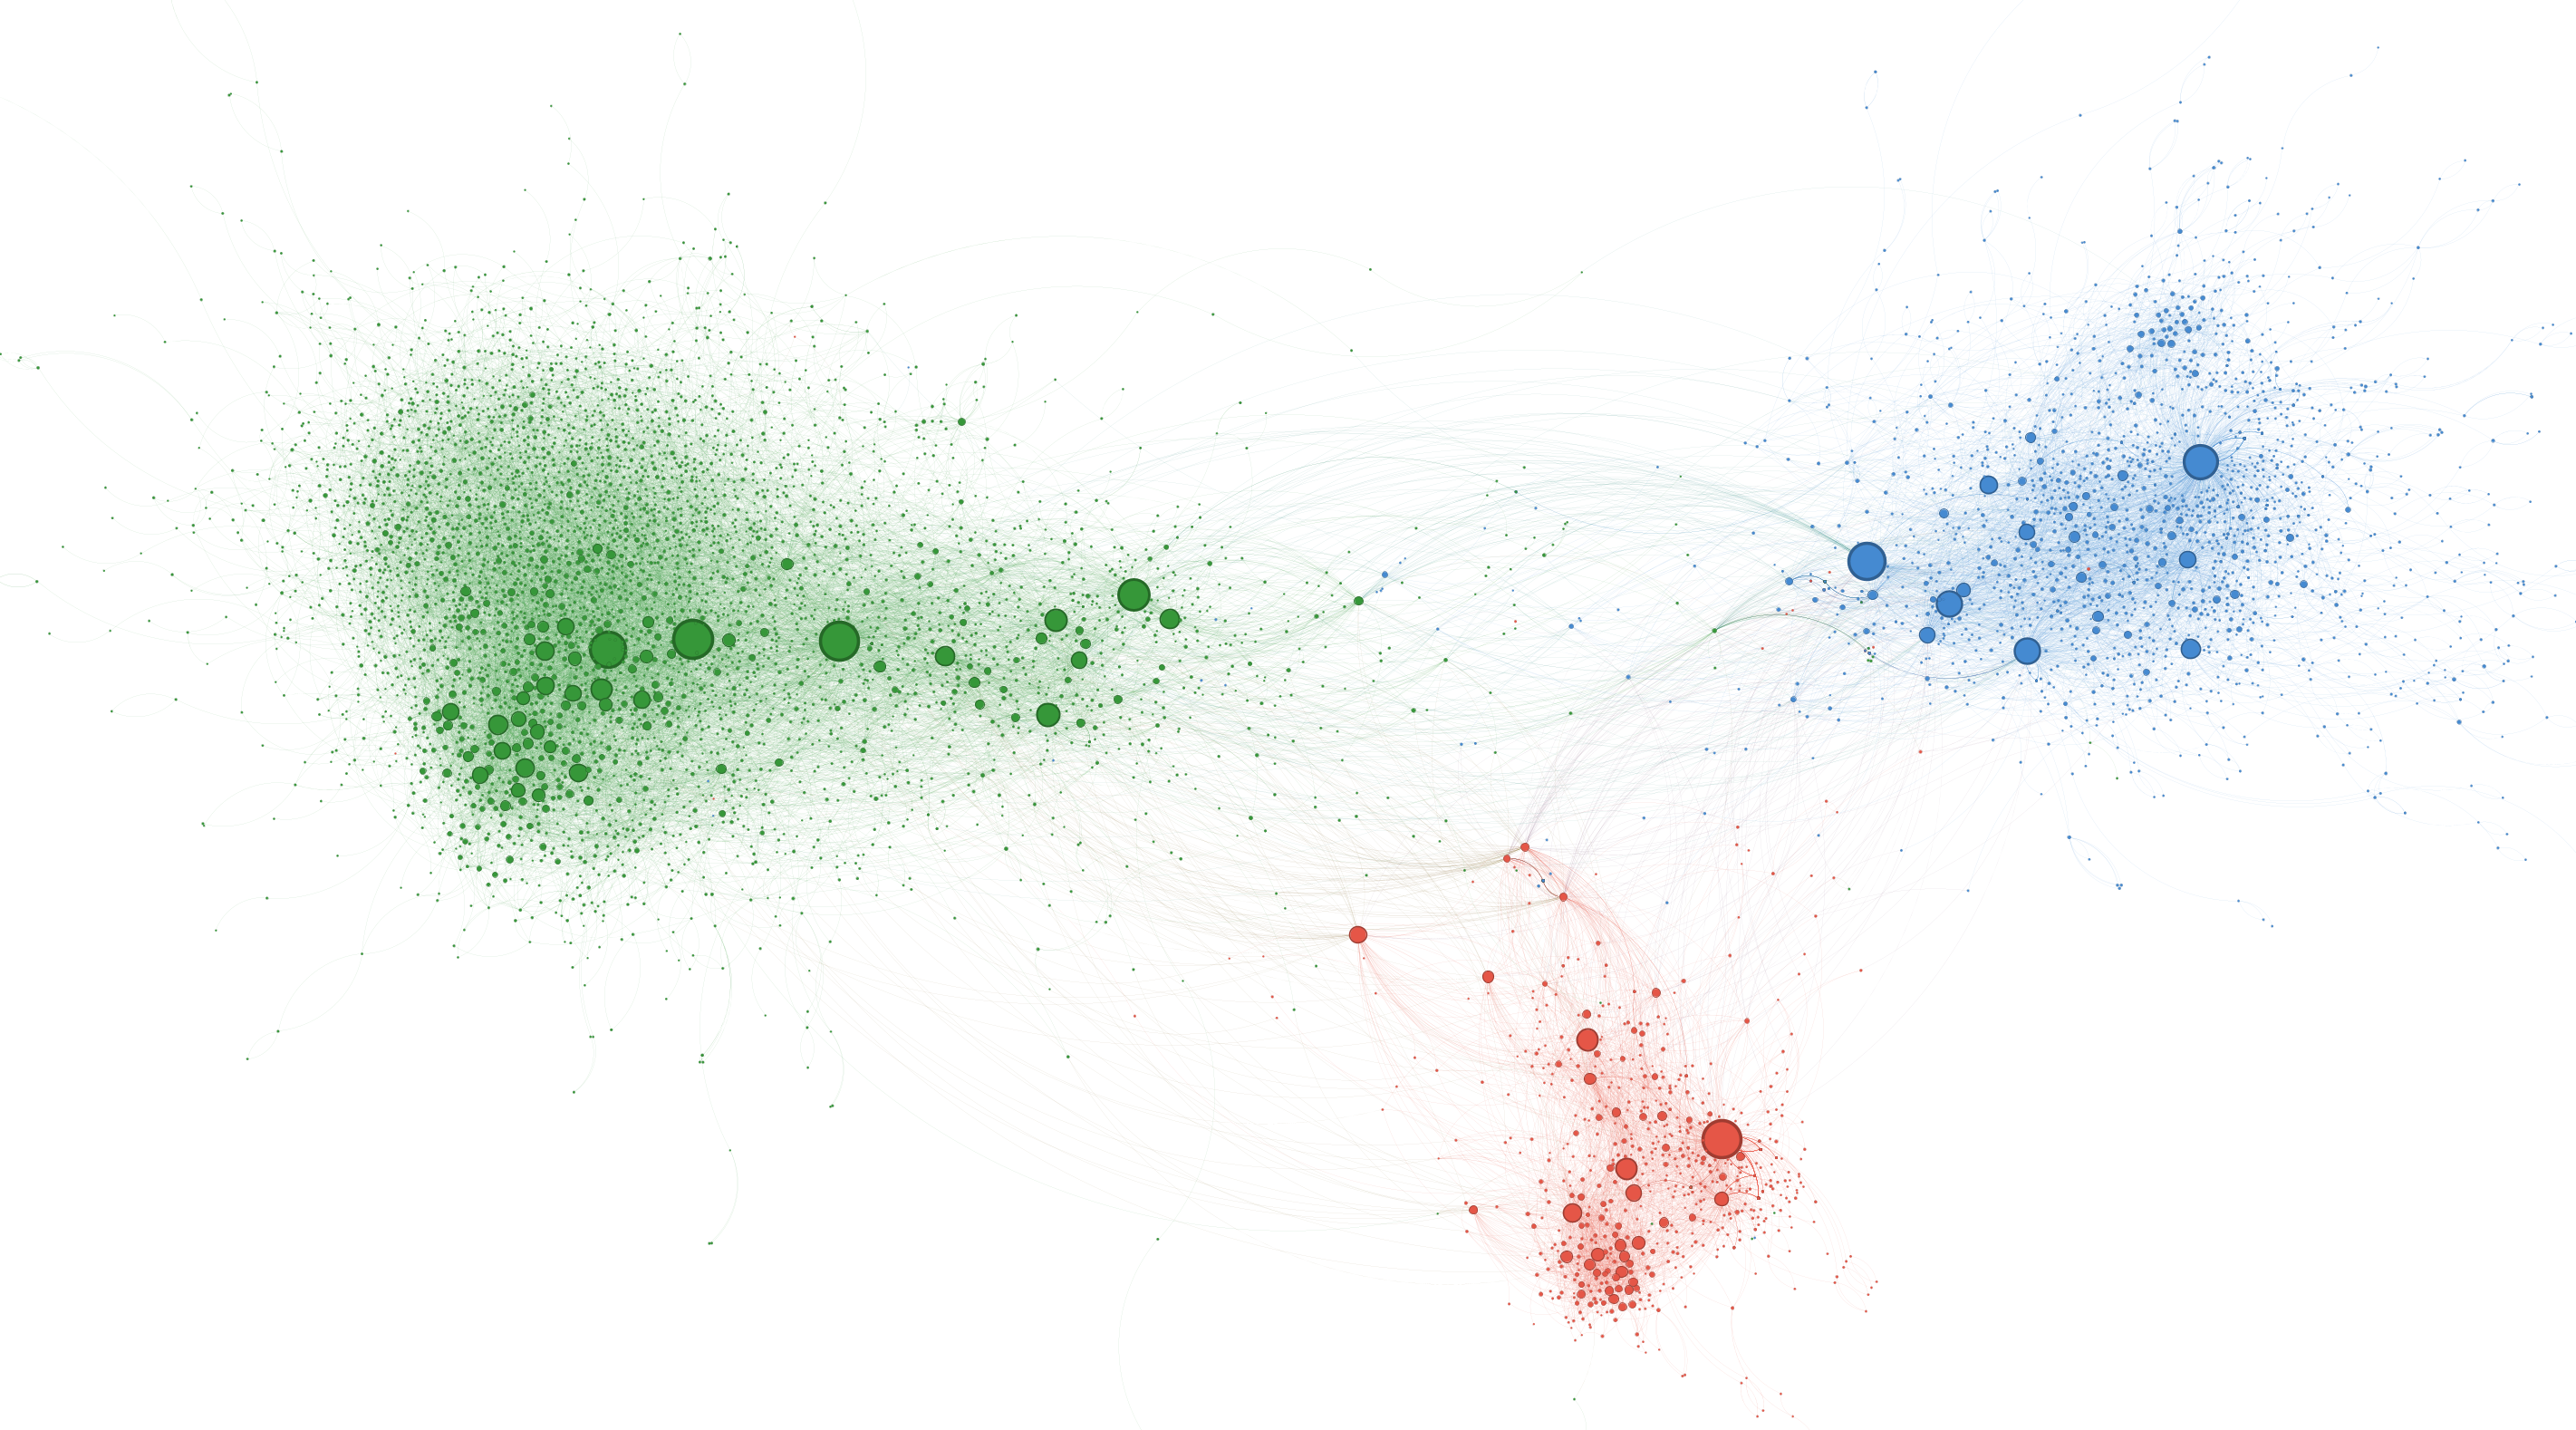
\includegraphics[scale=0.20]{images/colab_graph_3_cidades.png}
	\fautor
\end{figure}

Para iniciar, efetuamos uma filtragem dos dados, restringindo a análise aos usuários destas três cidades, resultando em uma rede composta por 6963 nós e 25785 arestas, uma redução significativa em comparação com os números iniciais de 33818 nós e 66875 arestas da rede original. Este processo de granulação permite uma análise mais focada e detalhada, facilitando a identificação de padrões e tendências específicas destas localidades.

Posteriormente, aplicamos um filtro adicional para considerar apenas os usuários com um grau de entrada maior que dois, visando eliminar nós isolados e focar em usuários com um mínimo de engajamento na rede. Além disso, focamos nossa análise no "Giant Component", que é a maior componente conectada da rede, onde existe um caminho entre cada par de nós. Este componente é crucial para entender a estrutura principal da rede, pois engloba a maior parte das interações significativas.

A coloração dos nós foi estabelecida de acordo com a cidade de origem dos usuários, adotando azul para Mesquita, rosa para Niterói e verde para Santo André, criando uma visualização que destaca a proveniência geográfica dos usuários. Adicionalmente, o tamanho dos nós foi ajustado com base no grau de entrada, representando a quantidade de seguidores, uma estratégia que realça os usuários mais influentes na rede.

Ao aplicar os layouts Force Atlas 2 e Yifan Hu, observamos uma separação natural da rede em três macro comunidades ou hubs, cada uma correlacionada a uma cidade específica. Este fenômeno evidencia um alto grau de homofilia pela localização, indicando que usuários tendem a interagir mais frequentemente com outros usuários da mesma cidade, um padrão que é corroborado em ambas as visualizações de layout, reforçando a validade desta observação.

\begin{figure}[!htb]
	\caption{Plot da rede utilizando o layout Yifan Hu.}
	\label{fig:colab_graph_3_cidades_yifan }
	\centering
	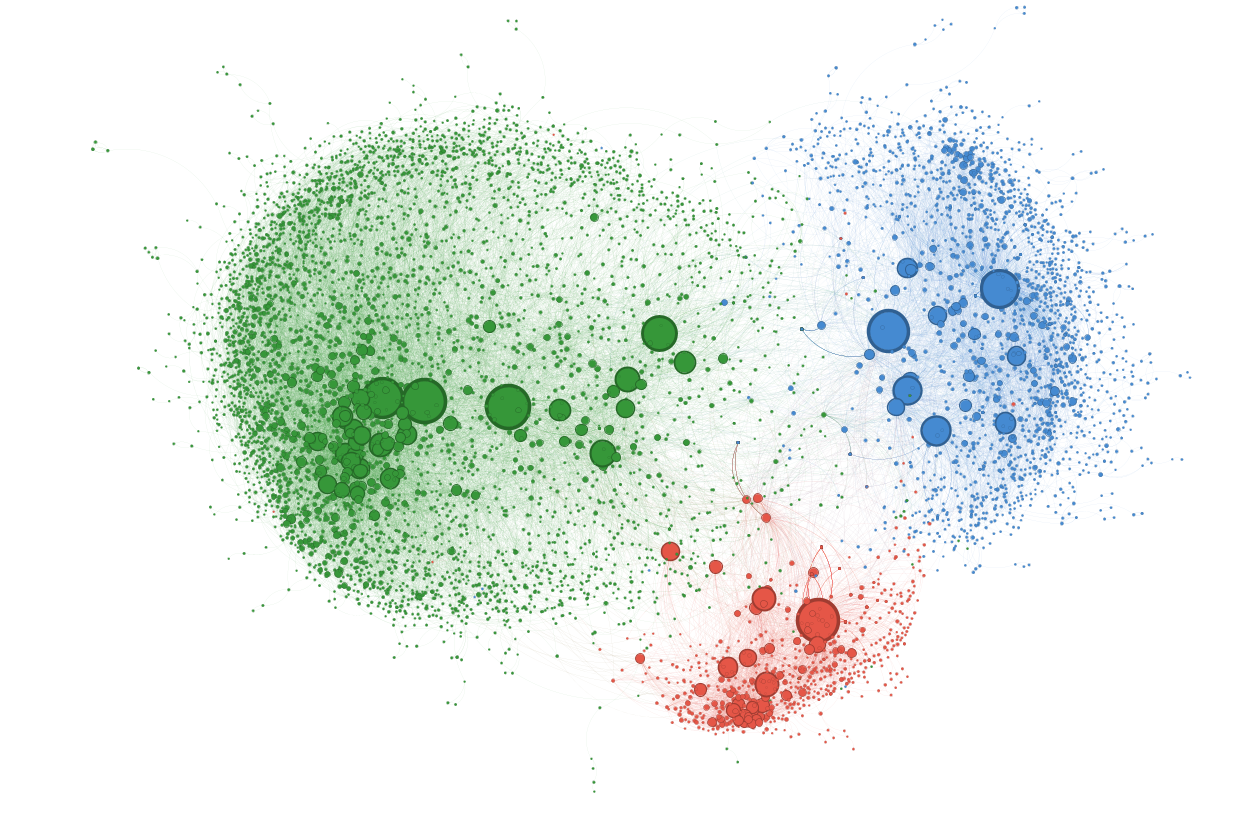
\includegraphics[scale=0.45]{images/colab_graph_3_cidades_yifan.png}
	\fautor
\end{figure}

Ao analisar as estatísticas da rede das três cidades, encontramos um grau médio de 3.703, indicando que, em média, cada usuário está conectado a aproximadamente 3-4 outros usuários. O diâmetro da rede, que é a maior distância entre dois nós, é 17, enquanto o comprimento médio do caminho é 5.318, sugerindo que, em média, são necessários pouco mais de cinco passos para conectar quaisquer dois usuários na rede. Este valor é uma indicação da eficiência da rede na disseminação de informações, onde valores menores indicam uma rede mais conectada e eficiente na transmissão de informações \cite{2010_Newman_BOOK}.

A modularidade encontrada foi de 0.519, um valor que indica uma estrutura de comunidade moderada, com uma presença significativa de grupos de usuários que estão mais densamente conectados entre si do que com o resto da rede. Este valor, juntamente com a presença de três hubs principais correlacionados com as cidades, sugere a existência de câmaras de eco geograficamente definidas, onde os usuários estão mais propensos a interagir e compartilhar informações com outros usuários de sua própria cidade, potencialmente levando a uma polarização e homogeneização de informações e perspectivas dentro dessas comunidades \cite{2010_Fortunato}.

A inferência estatística apresentou um valor de 193900.35, um indicador que, embora seja mais desafiador interpretar isoladamente, sugere uma complexidade considerável na estrutura da rede, com uma grande quantidade de comunidades distintas e padrões de conexão. Este valor, juntamente com o número significativo de componentes conectados (69 fracamente e 3927 fortemente), indica uma rede com uma estrutura complexa e multifacetada, com muitos subgrupos e comunidades interconectadas.

A centralidade de eigenvector, com uma mudança somatória de 0.015, aponta para a presença de nós influentes que desempenham um papel significativo na estrutura da rede. Estes nós, que são centrais em termos de eigenvector, podem atuar como "líderes de opinião" ou influenciadores dentro de suas respectivas comunidades, desempenhando um papel crucial na disseminação de informações e na formação de opiniões \cite{1987_Bonacich}.

Em conclusão, a análise da rede das três cidades revela uma estrutura complexa e interconectada, com padrões claros de homofilia geográfica e a presença de comunidades densamente conectadas. A combinação de visualizações de layout, métricas de rede e análises estatísticas fornece insights valiosos sobre a natureza das interações entre os usuários e as potenciais câmaras de eco que se formam dentro desta rede.

Na sequência de nossa análise, realizamos uma filtragem meticulosa dos dados no Gephi para refinar nossa visualização e focar nas interações mais significativas. Esta etapa é crucial para eliminar ruídos e destacar as estruturas subjacentes que são mais informativas. Após a filtragem, aplicamos uma coloração baseada na 'Modularidade de Classe', uma métrica que quantifica a densidade de ligações dentro das comunidades em comparação com as ligações entre comunidades. Valores altos de modularidade indicam uma divisão clara da rede em comunidades. O algoritmo de detecção de comunidades do Gephi é baseado no trabalho de \citeonline{2008_Blondel}.

\begin{table}[h]
	\centering
	\begin{tabular}{lccc}
		\hline
		\textbf{Métrica}      & \textbf{Mesquita} & \textbf{Niterói} & \textbf{Santo André} \\
		\hline
		Nodes                 & 718               & 4272             & 1973                 \\
		Edges                 & 3208              & 15751            & 6101                 \\
		Average Degree        & 4.468             & 3.687            & 3.092                \\
		Diameter              & 8                 & 16               & 13                   \\
		Average Path length   & 3.142             & 4.977            & 4.088                \\
		Modularity            & 0.310             & 0.438            & 0.411                \\
		Number of Communities & 32                & 75               & 87                   \\
		\hline
	\end{tabular}
	\caption{Estatísticas das redes das cidades de Mesquita, Niterói e Santo André.}
\end{table}

Em nossa análise de rede, priorizamos as três cidades com maior volume de interações no Colab: Niterói, Santo André e Mesquita. Avaliando a mediana dos atributos de cada cidade, Mesquita se destaca em termos de centralidade de grau e de eigenvector.

No contexto das três cidades analisadas, a métrica de modularidade revela informações cruciais sobre a estrutura da rede. Por exemplo, uma modularidade elevada sugere que a rede tem uma estrutura comunitária bem definida, o que pode ser indicativo de câmaras de eco. A detecção de comunidades e a análise da modularidade, portanto, fornecem uma lente através da qual podemos observar a formação de câmaras de eco. Em Mesquita, Niterói e Santo André, as métricas de modularidade indicam a presença de comunidades distintas. Estas comunidades, quando analisadas em detalhe, podem revelar padrões de interação que são característicos de câmaras de eco. Por exemplo, se uma comunidade particular é dominada por um único tópico de discussão ou por uma perspectiva única, isso pode ser um sinal de uma câmara de eco em ação.

Estas técnicas nos permitiram visualizar claramente as diferentes comunidades dentro de cada cidade, destacando a estrutura interna e as possíveis câmaras de eco. Em vez do algoritmo 'Force Atlas 2', optamos pelo algoritmo de layout 'Fruchterman-Reingold'. Este método, frequentemente descrito como "baseado em forças", simula uma situação em que os nós se repulsam mutuamente, como partículas carregadas negativamente, enquanto as arestas que os conectam atuam como molas, buscando manter os nós a uma distância desejada. O algoritmo move os nós de acordo com essas forças até que um equilíbrio seja alcançado, proporcionando uma representação visual clara e intuitiva das comunidades e suas inter-relações.

\begin{figure}[h]
    \centering
    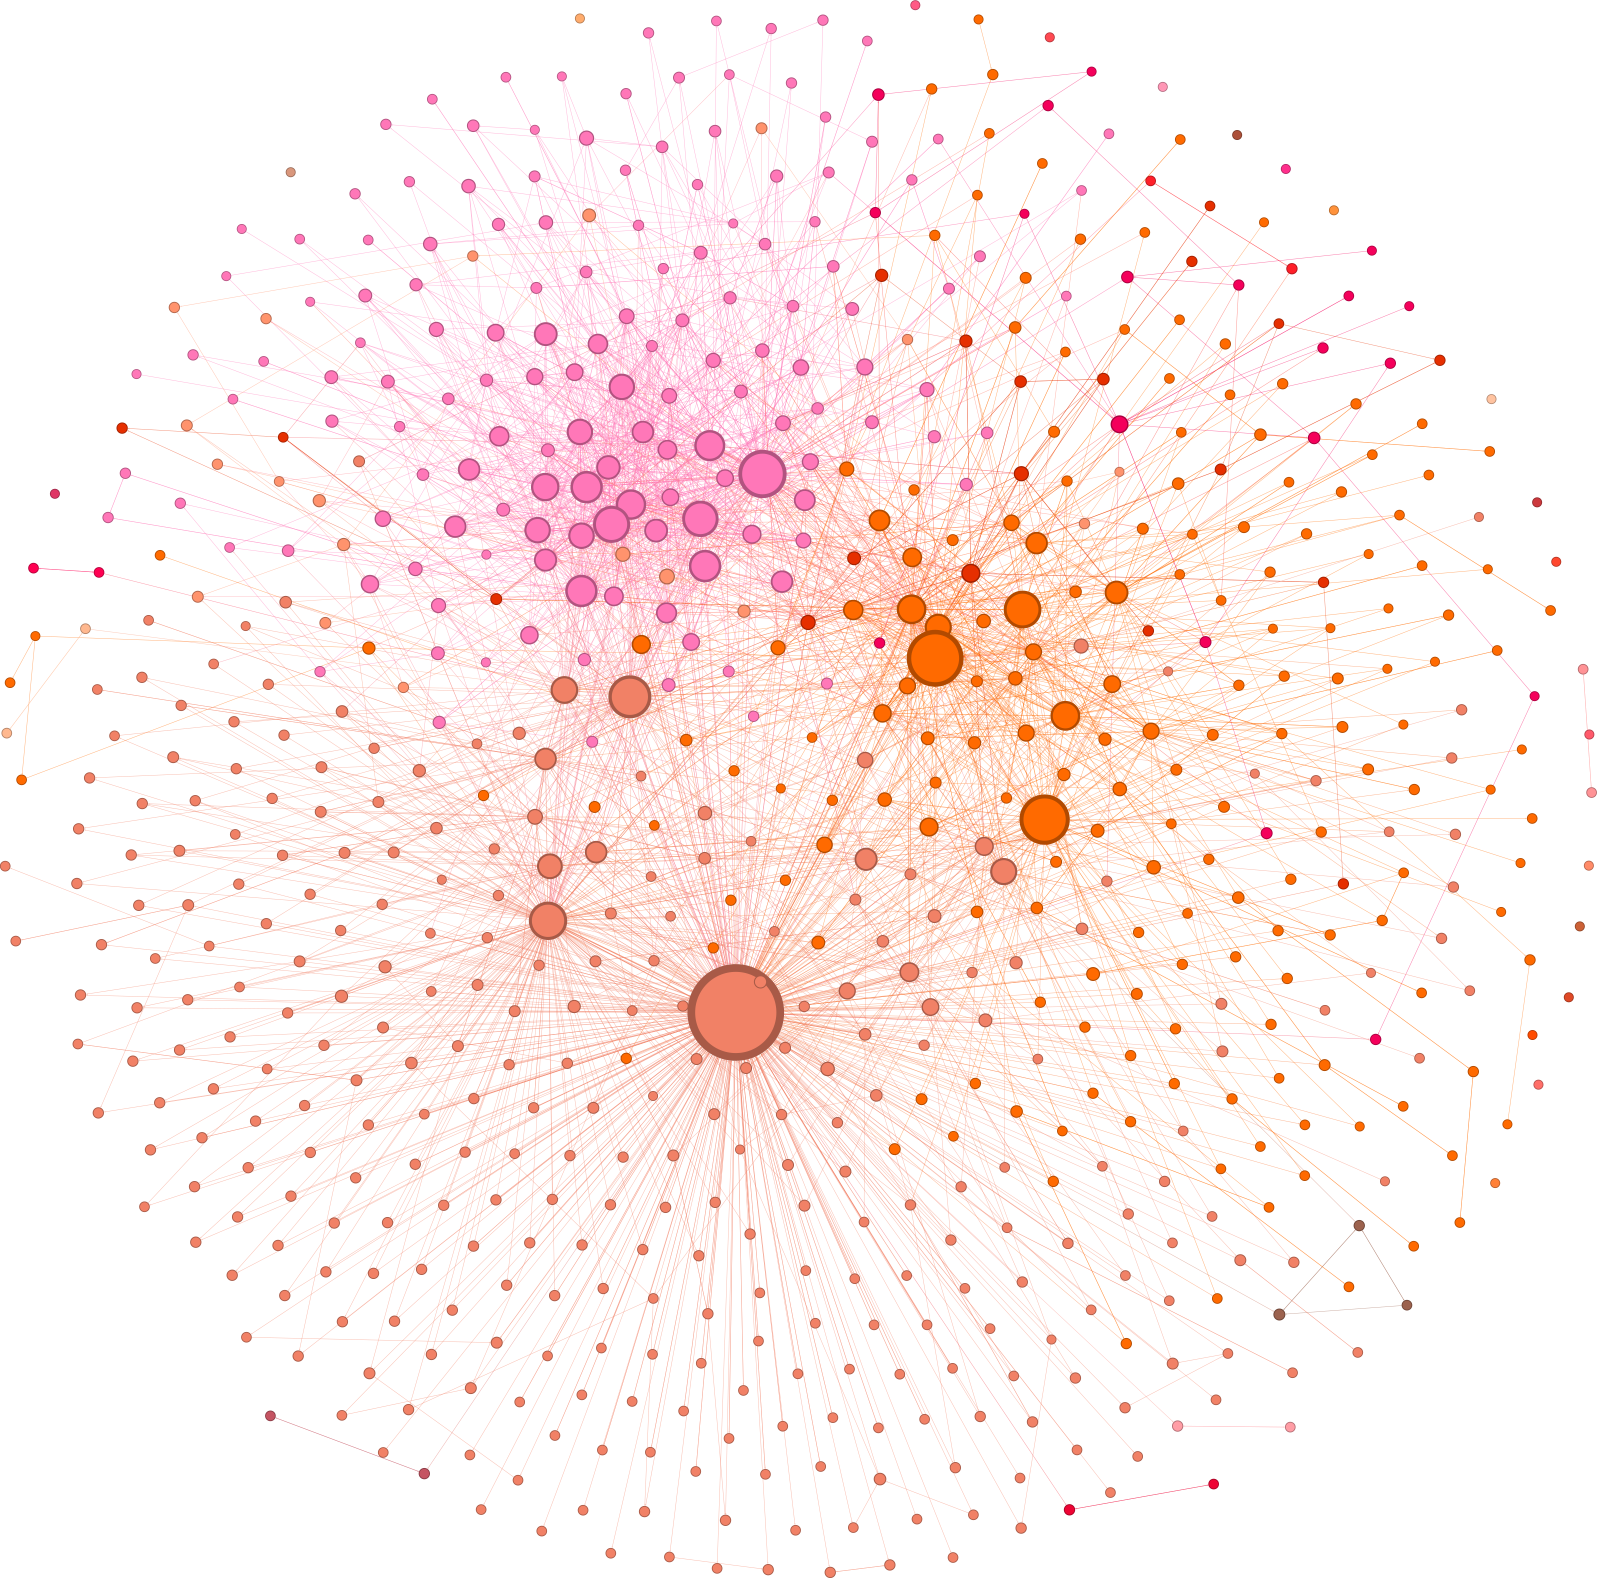
\includegraphics[width=0.8\textwidth]{images/graph-mesquita.png}
    \caption{Visualização da rede da cidade de Mesquita. O layout foi gerado usando o algoritmo Fruchterman-Reingold e o agrupamento foi realizado com o método de Louvain.}
    \label{fig:mesquita-graph}
	\fautor
\end{figure}

Na cidade de Mesquita, a rede é composta por 718 nós e 3208 arestas, com um grau médio de 4.468. O diâmetro da rede é de 8, indicando que o caminho mais longo entre dois nós é de 8 arestas. A métrica de 'Modularidade' é de 0.310, sugerindo uma presença moderada de comunidades dentro da rede. A detecção de comunidades revelou 32 comunidades, enquanto a inferência estatística sugere a existência de 75 comunidades. Esta discrepância pode ser devido a diferentes métodos de detecção de comunidades ou a presença de subcomunidades dentro das principais comunidades identificadas. A presença de 21 componentes fracamente conectados e 315 componentes fortemente conectados indica que, embora existam muitos grupos isolados, a maioria dos nós está fortemente interconectada.

\begin{figure}[h]
    \centering
    \includegraphics[width=0.8\textwidth]{images/graph-niteroi.png}
    \caption{Visualização da rede da cidade de Niterói. O layout foi gerado usando o algoritmo Fruchterman-Reingold e o agrupamento foi realizado com o método de Louvain.}
    \label{fig:niteroi-graph}
	\fautor
\end{figure}

Em Niterói, a rede é significativamente maior, com 4272 nós e 15751 arestas. O grau médio é de 3.687, e o diâmetro da rede é de 16. A 'Modularidade' é de 0.438, indicando uma presença mais forte de comunidades em comparação com Mesquita. Foram identificadas 75 comunidades, e a inferência estatística sugere a presença de 316 comunidades. O coeficiente de agrupamento médio é de 0.086, o que sugere que os nós tendem a criar triângulos ou tríades. Esta métrica é importante porque indica a tendência dos nós de formar grupos fechados, o que pode ser um indicativo da formação de câmaras de eco.

\begin{figure}[h]
    \centering
    \includegraphics[width=0.8\textwidth]{images/graph-santo-andre.png}
    \caption{Visualização da rede da cidade de Santo André. O layout foi gerado usando o algoritmo Fruchterman-Reingold e o agrupamento foi realizado com o método de Louvain.}
    \label{fig:santo-andre-graph}
	\fautor
\end{figure}

Santo André apresenta uma rede com 1973 nós e 6101 arestas. O grau médio é de 3.092, e o diâmetro da rede é de 13. A 'Modularidade' é de 0.411, sugerindo uma presença forte de comunidades. Foram identificadas 87 comunidades, enquanto a inferência estatística sugere a existência de 164 comunidades. O coeficiente de agrupamento médio é de 0.220, o que é significativamente maior do que em Niterói, indicando uma maior tendência dos nós em Santo André de formar grupos fechados.

A detecção de comunidades é uma área de pesquisa em rápido crescimento, com aplicações em várias disciplinas, desde a biologia até as ciências sociais. Segundo \citeonline{2010_Fortunato}, a capacidade de identificar comunidades em redes complexas permite uma melhor compreensão da estrutura e função dessas redes. Em relação às câmaras de eco online, \citeonline{2016_Vicario} destacam que as redes sociais online podem amplificar a polarização e a segregação, levando à formação de câmaras de eco onde os usuários são expostos principalmente a informações que reforçam suas crenças preexistentes.

A presença de comunidades densamente conectadas e a formação de câmaras de eco são fenômenos inter-relacionados. As comunidades tendem a formar-se em torno de interesses ou opiniões comuns, e dentro dessas comunidades, os membros são mais propensos a interagir com informações que confirmam suas crenças, levando à formação de câmaras de eco. Este fenômeno é exacerbado pelas plataformas de mídia social que utilizam algoritmos de recomendação para mostrar aos usuários conteúdo que é provável que eles achem interessante ou concordem, reforçando ainda mais as câmaras de eco.

Ao examinar a estrutura da rede em Mesquita, observamos um padrão distintivo: um usuário em particular emerge como uma figura central, atuando como um hub com múltiplas conexões irradiando a partir dele. Em contraste, Santo André exibe uma configuração mais fragmentada, caracterizada por diversos núcleos descentralizados. Niterói, contudo, diverge desses padrões, manifestando uma rede compacta e coesa, onde as conexões são densamente entrelaçadas.

Ao mergulhar nas métricas da rede, notamos que Mesquita ostenta uma predominância de usuários cujo eigenvector é marginalmente elevado. Em contrapartida, tanto Santo André quanto Niterói apresentam uma distribuição onde a maioria dos usuários tem um eigenvector aproximando-se de zero.

Em uma perspectiva sobre a demografia dos usuários, correlacionando-os com o valor do eigenvector percebe-se que em Niterói, uma demografia mais jovem é evidente, uma característica que não é tão proeminente em Mesquita ou Santo André. Em uma observação mais ampla, os usuários que detêm uma centralidade elevada tendem a ter idades entre 31 e 64 anos.

Explorando ainda mais a arquitetura das redes, nos deparamos com o conceito de excentricidade. Esta métrica delineia a distância máxima entre um nó específico e todos os demais na rede. Em termos mais coloquiais, a excentricidade de um nó representa a distância mais longa, contada pelo número de arestas, que se deve percorrer para alcançar esse nó a partir de qualquer outro ponto da rede.

A investigação da rede social Colab desvelou nuances sobre a dinâmica e o perfil dos usuários. Uma constatação notável é que a vasta maioria dos usuários mantém até 10 conexões, tendo registrado até 10 comentários e 10 curtidas.

Ao focar nos usuários mais proeminentes, identificamos uma demografia que oscila entre 37 e 52 anos. Globalmente, a plataforma é dominada por indivíduos do sexo masculino, de etnia branca e com formação acadêmica avançada.

Ao segmentar os usuários em cinco clusters através do K-means, percebemos que Mesquita e Santo André exibem padrões distributivos análogos, enquanto Niterói se distingue com um cluster particularmente proeminente. Notavelmente, o cluster composto por indivíduos de maior influência permeia as três cidades, com uma representatividade mais acentuada em Mesquita.

Em um esforço para mapear a distribuição geográfica dos clusters, não identificamos aglomerações em áreas específicas das cidades.

Ao focar exclusivamente nas conexões entre usuários, geramos visualizações das redes. Em Mesquita, uma concentração de usuários em torno de um indivíduo é patente, com o restante da rede apresentando-se mais disperso. Em Santo André, a rede é pontuada por diversos núcleos menores. Em Niterói, a representação gráfica revela uma rede intrincada e coesa.

Concluindo, nossa incursão na análise da rede social do Colab nos brindou com insights profundos sobre as interações dos usuários, a dinâmica da plataforma e os perfis dos usuários mais influentes. Estes achados iniciais sobre a rede Colab são cruciais para orientar aprimoramentos na plataforma, potencializar a interação entre os usuários, conceber estratégias de comunicação mais eficazes e prover informações valiosas aos stakeholders.

À luz da metodologia de \citeonline{2023_Atiqi_BOOK}, a topologia das redes das 3 cidades, sugere a presença de subgrupos ou comunidades que podem funcionar como câmaras de eco. Estas são áreas da rede onde os membros estão fortemente alinhados em suas opiniões ou informações compartilhadas. A presença de múltiplos componentes fortemente conectados em cada cidade indica que, enquanto há muita interconexão, também existem bolsões isolados de opinião. Estes bolsões podem ser áreas onde as opiniões são reforçadas sem exposição a perspectivas divergentes, um indicativo clássico de câmaras de eco. A modelagem baseada em agentes, como proposto por Atiqi, pode ajudar a entender melhor como as informações se propagam nessas redes e como as câmaras de eco se formam e persistem.

Em conclusão, a análise das redes das três cidades revela padrões distintos de interconexão e formação de comunidades. A presença de comunidades densamente conectadas sugere a possibilidade de câmaras de eco, onde os membros são expostos a um conjunto limitado de informações que reforçam suas crenças preexistentes. Esta análise destaca a importância de compreender a estrutura e dinâmica das redes sociais para abordar os desafios associados à polarização e segregação online.

\subsection*{Limitações do algoritmo de Louvain}
\label{sec:limitacoes_louvain}

É importante destacar que o algoritmo de Louvain foi originalmente desenvolvido para redes não direcionadas. No entanto, muitas redes reais, incluindo a rede que estamos analisando neste estudo, são direcionadas. Neste contexto, uma questão pertinente surge: como o Gephi, que utiliza o algoritmo de Louvain, lida com redes direcionadas?

Ao analisar o código fonte \cite{2011_McSweeney} e os relatórios gerados pelo Gephi, observa-se que a ferramenta parece converter redes direcionadas em não direcionadas para a aplicação do algoritmo de Louvain. Essa abordagem, embora permita a utilização de uma metodologia consolidada de detecção de comunidades, pode não capturar completamente a estrutura e as nuances de uma rede direcionada. Por exemplo, relações de autoridade, hierarquia ou influência, que são intrínsecas a redes direcionadas, podem ser perdidas durante essa conversão.

Além da metodologia de Louvain tradicionalmente aplicada a redes não direcionadas, é essencial considerar a dinâmica e a estrutura modular em múltiplas escalas em redes. \citeonline{2008_Lambiotte} destaca que muitas redes são inerentemente modulares, o que significa que elas consistem em módulos ou comunidades. A estabilidade, definida pelas propriedades estatísticas de um caminhante aleatório movendo-se no gráfico, é usada como uma medida para determinar a qualidade de uma partição. Uma observação crítica é que a estabilidade da partição de um gráfico muda com o tempo, permitindo uma compreensão em várias escalas das comunidades em redes. No entanto, uma consideração crucial é que a modularidade e a estabilidade são fundamentalmente diferentes no caso de redes direcionadas. Isso sugere que, ao aplicar métodos como o de Louvain a redes direcionadas, como as encontradas em muitos contextos de mídia social, é vital considerar essas diferenças e as implicações metodológicas resultantes.

\subsection*{Alternativas em detecção de comunidades}

Ao abordar redes direcionadas, é crucial considerar a direcionalidade das arestas. Como discutido por \citeonline{2013_Malliaros}, ignorar essa direcionalidade pode levar à perda de semântica subjacente. Em muitos casos, essa simplificação não seria satisfatória, especialmente em redes onde a direcionalidade tem um significado significativo. Além disso, a presença de arestas direcionadas implica a possibilidade de tipos mais sofisticados de clusters que representam padrões de movimento ou circulação de fluxo entre os nós. Portanto, ao aplicar métodos como o Louvain em redes direcionadas, é essencial adaptar e considerar essas nuances para garantir que as comunidades detectadas sejam verdadeiramente representativas da estrutura da rede.

Uma alternativa ao cálculo de modularidade padrão do Gephi é o algoritmo de Girvan-Newman, proposto por \cite{2002_Girvan}. Este algoritmo é baseado na ideia de que uma aresta entre duas comunidades tem, provavelmente, menos ligações do que uma aresta dentro de uma comunidade. Assim, ao remover iterativamente as arestas com a maior centralidade de intermediação (ou "betweenness"), as comunidades emergem naturalmente como componentes desconexos. O algoritmo é particularmente eficaz em redes com estrutura hierárquica de comunidades e tem sido amplamente utilizado em diversos campos de pesquisa.

Através de um plugin para o Gephi, é possivel aplicar o algoritmo de Girvan-Newman à rede de Mesquita, por exemplo, encontramos um total de 67 comunidades, com uma modularidade máxima de 0.3027. Em contraste, o cálculo de modularidade padrão do Gephi identificou 26 comunidades com uma modularidade de 0.431. A diferença na quantidade de comunidades e nos valores de modularidade sugere que os dois métodos têm diferentes sensibilidades à estrutura da rede. No contexto da nossa pesquisa sobre câmaras de eco, a escolha do método pode depender do foco da análise. Se estivermos interessados em identificar um maior número de comunidades potencialmente menores e mais coesas, o algoritmo de Girvan-Newman pode ser mais apropriado. No entanto, se buscarmos uma visão mais macroscópica das principais comunidades na rede, a abordagem de modularidade padrão do Gephi pode ser preferível. Ambos os métodos oferecem insights valiosos, e a escolha pode ser guiada pelo objetivo específico da análise e pela natureza da rede em estudo.

O algoritmo Leiden, uma extensão avançada do método de Louvain, é uma abordagem contemporânea para detecção de comunidades em redes \cite{2018_Traag}. Desenvolvido para superar certas limitações do Louvain, o Leiden opera através de um processo iterativo de particionamento local, refinamento e agregação, garantindo uma partição de alta qualidade ao otimizar a modularidade da rede. Em nossa análise para a cidade de Mesquita, utilizando o algoritmo Leiden com a função de qualidade baseada em modularidade e uma resolução de 1.0 ao longo de 100 iterações, obtivemos uma modularidade de 0.4441 e identificamos 30 comunidades distintas. Em comparação com os resultados anteriores, o Leiden apresentou uma modularidade ligeiramente superior ao método padrão do Gephi (0.431) e identificou um número de comunidades que se situa entre o método padrão do Gephi (26 comunidades) e o Girvan-Newman (67 comunidades). Essa variação nos resultados destaca a sensibilidade dos diferentes algoritmos à estrutura da rede e reforça a importância de considerar múltiplas abordagens ao analisar comunidades em redes complexas.

No entanto, a pesquisa está avançando para superar essa limitação. O estudo de \citeonline{2015_Dugue} introduz uma extensão do método de Louvain para redes direcionadas, preservando a direcionalidade das conexões na análise de comunidades. Essa abordagem, denominada DirectedLouvain, maximiza uma função objetivo de modularidade direcionada, permitindo a detecção de comunidades em redes com links direcionados. A implementação dessa metodologia pode oferecer insights mais profundos sobre a estrutura da rede, mantendo a riqueza de informações contida nas direções dos links. Assim, para estudos futuros, seria interessante explorar a aplicação do DirectedLouvain para uma análise mais refinada das câmaras de eco, levando em consideração a direcionalidade das conexões na rede.

\section{Abordagem programática}

\begin{figure}[h]
    \centering
    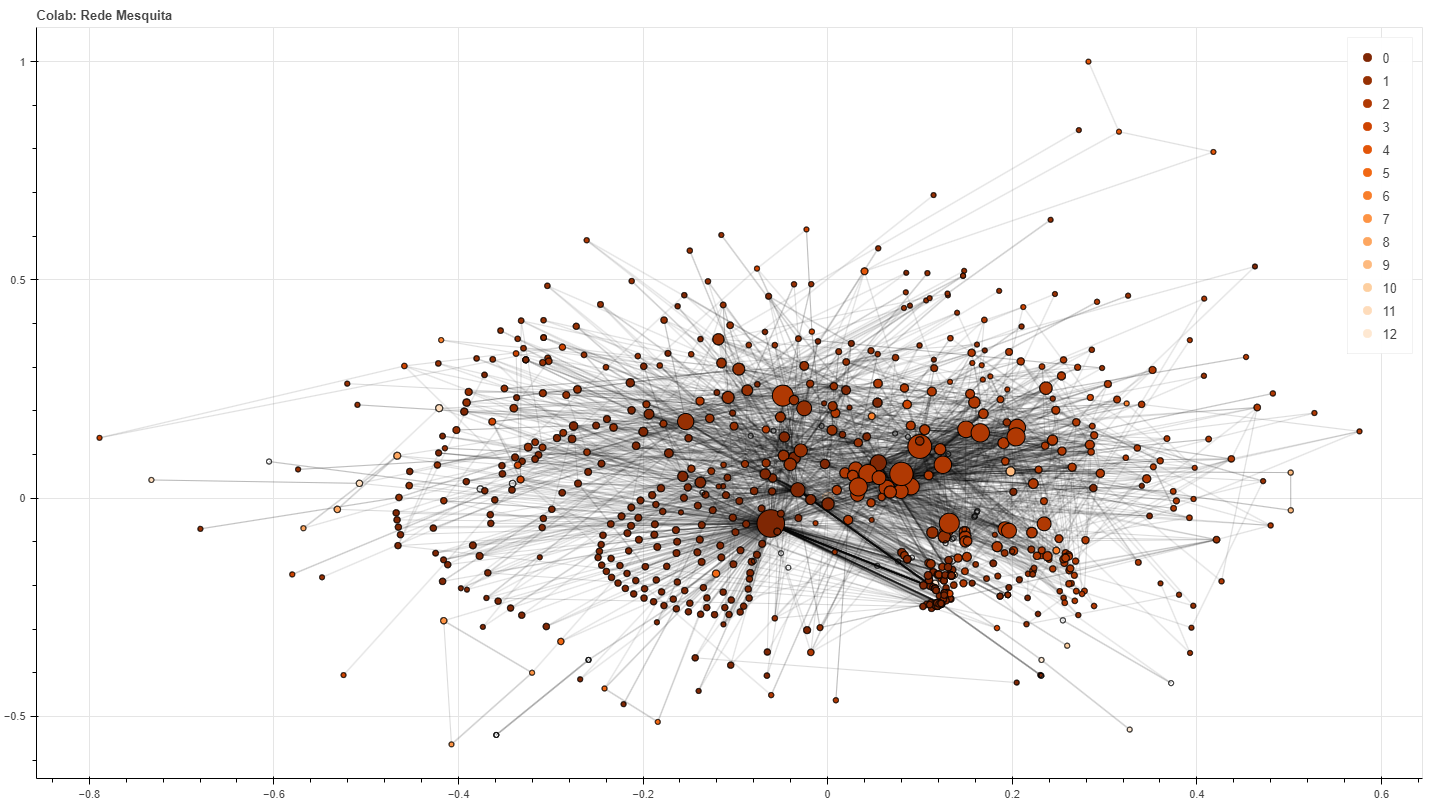
\includegraphics[scale=0.30]{images/bokeh_plot.png}
    \caption{Visualização interativa da rede Colab na cidade de Mesquita utilizando a biblioteca Bokeh. Layout aplicado: Kamada-Kawai.}
    \label{fig:bokeh_plot}
	\fautor
\end{figure}

Durante nossa análise exploratória da rede social do Colab, inicialmente optamos por utilizar a ferramenta Gephi para visualização e análise dos dados. Utilizando o Gephi, conseguimos identificar algumas características interessantes da rede, como agrupamentos e centralidades. No entanto, conforme a complexidade da rede aumentava, percebemos que o processo de análise manual no Gephi se tornava mais desafiador e demorado. Além disso, a reprodução dos passos de análise no Gephi era difícil de compartilhar e replicar. Por fim, como discutido acima, as heurísticas de modularidade do Gephi não são adequadas para redes direcionadas, o que não é neccessariamente um problema em uma análise a nível exploratório, mas que pode ser relevante ao se tratar de heurísticas para detecção de câmaras de eco baseado em comunidades de um grafo.

Para superar essas limitações, decidimos incorporar uma abordagem baseada em código em nossa análise. Isso nos permitiu automatizar várias etapas do processo de análise, proporcionando uma maior flexibilidade e eficiência. Em particular, desenvolvemos uma classe chamada NetworkPlotter em Python, que nos permitiu realizar análises mais avançadas e explorar diferentes métricas de SNA.

A abordagem baseada em código nos trouxe diversos benefícios em relação ao uso do Gephi. Em primeiro lugar, a automação das etapas de análise nos permitiu trabalhar com redes maiores e mais complexas, que seriam impraticáveis de analisar manualmente no Gephi. Além disso, a flexibilidade do código nos permitiu ajustar e personalizar as análises de acordo com nossas necessidades específicas. Também pudemos criar visualizações interativas dos resultados, permitindo uma exploração mais profunda da rede.

A classe NetworkPlotter foi essencial nesse processo. Ela encapsula a lógica para a visualização e análise de redes complexas, utilizando bibliotecas como NetworkX e Bokeh. A classe nos permite calcular métricas de grau e centralidade, normalizar tamanhos de nós e criar visualizações interativas do grafo. Essa abordagem orientada a código nos forneceu uma ferramenta poderosa e reutilizável para análise de redes sociais, facilitando a exploração e compreensão da estrutura e dinâmica da rede do Colab.

Iniciando com a métrica de grau, é utilizado o método \texttt{nx.degree()} para calcular o grau de cada nó, representando o número de conexões de entrada ou saída do mesmo. Essa métrica permite identificar nós importantes dentro da rede, uma vez que nós com um alto grau estão mais conectados a outros nós e podem desempenhar papéis de influência significativos.

Além disso, o código emprega o algoritmo \texttt{nx.eigenvector\_centrality\_numpy()} para calcular a centralidade de cada nó. A centralidade de um nó mede sua importância relativa com base em sua posição e conexões no grafo. Nesse caso, o algoritmo de centralidade de eigenvector é utilizado para considerar tanto as conexões diretas de um nó quanto a importância dos nós vizinhos. Dessa forma, a centralidade pode ser interpretada como um indicador de influência ou prestígio dentro da rede.

Uma etapa adicional do código é a normalização do tamanho dos nós, realizada por meio da função \texttt{normalize()}. Essa normalização tem como objetivo ajustar visualmente os tamanhos dos nós com base em limites desejados e atuais, visando uma representação adequada no gráfico de rede. Essa técnica permite destacar visualmente os nós mais importantes com base em suas métricas de grau e centralidade, facilitando a análise e interpretação dos resultados.

\begin{figure}[h]
    \centering
    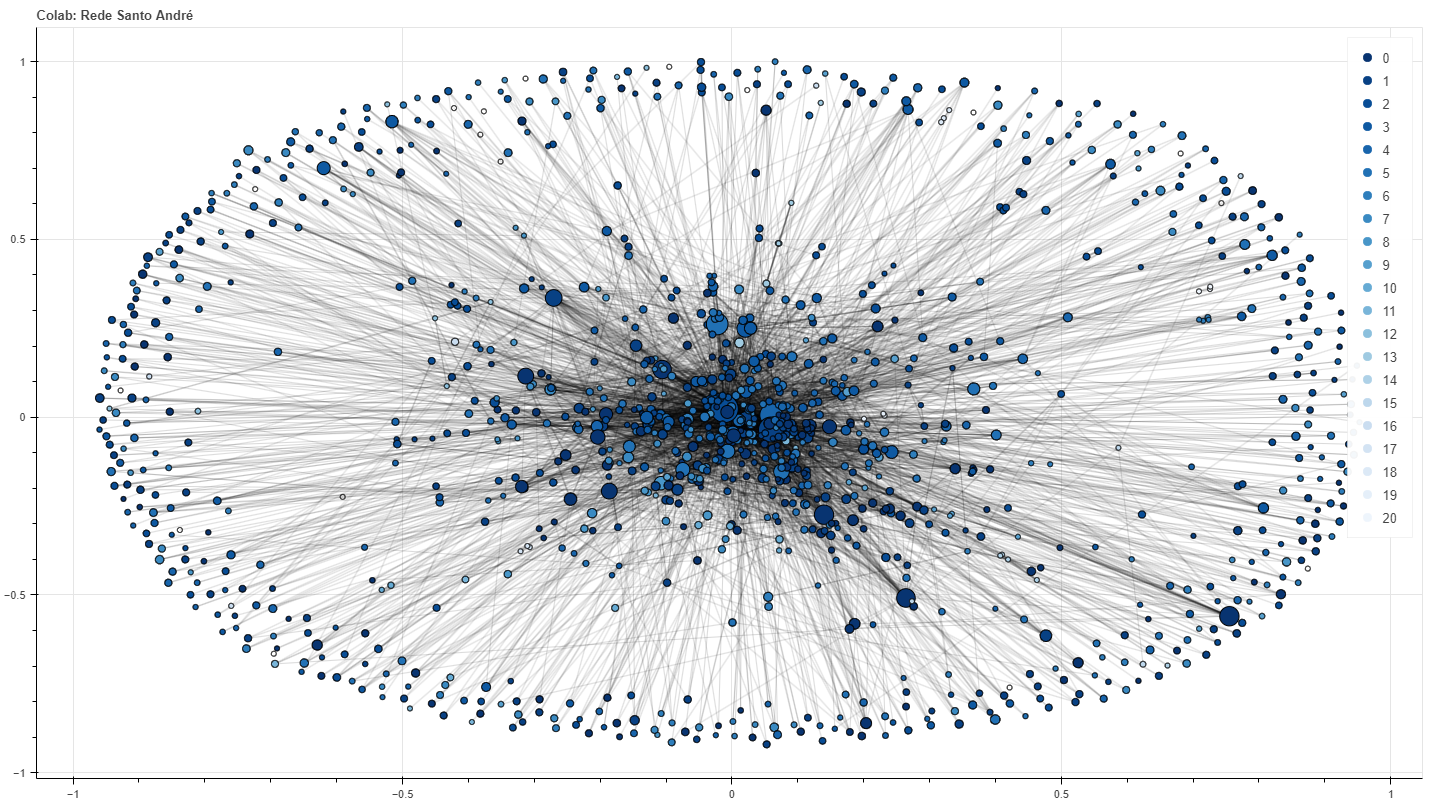
\includegraphics[scale=0.3]{images/bokeh_plot_santo_andre.png}
    \caption{Visualização interativa da rede Colab na cidade de Santo André com o layout spring, o padrão da biblioteca NetworkX.}
    \label{fig:bokeh_plot_santo_andre}
	\fautor
\end{figure}

Como ja discutido em \autoref{sec:limitacoes_louvain}, a detecção de comunidades em grafos direcionados é uma questão delicada que exige alguns benchmarks. Ao explorar diferentes métodos de detecção de comunidades, observamos variações significativas nos resultados, refletindo as diferentes abordagens e heurísticas que cada algoritmo utiliza. A abordagem de Louvain, por exemplo, identificou 116 comunidades na rede da cidade de Mesquita, com a maior comunidade composta por 118 nós e a menor por apenas um nó. A média de tamanho da comunidade foi de aproximadamente 6,19 nós, e o score de modularidade foi de 0,3574.

Por outro lado, o algoritmo de modularidade gananciosa \cite{2004_Clauset} identificou 40 comunidades, com a maior comunidade contendo 333 nós e a menor apenas um nó. A média de tamanho da comunidade foi significativamente maior, com cerca de 17,95 nós por comunidade, e um score de modularidade de 0,4297. No entanto, é importante observar que comunidades com apenas um ou dois nós podem não ser representativas ou significativas em muitos contextos de análise de redes sociais. Portanto, como etapa de pré-processamento, optamos por considerar apenas as comunidades que continham no mínimo 3 usuários. Esse critério visa garantir que as comunidades identificadas sejam robustas e tenham relevância prática, evitando a inclusão de pequenos agrupamentos que podem surgir devido a ruídos ou conexões esporádicas na rede. Ao aplicar esse filtro, o número total de comunidades e a distribuição de seus tamanhos podem variar, mas a análise resultante tende a ser mais focada em agrupamentos significativos e bem definidos na rede.

Comparando com os resultados obtidos no Gephi, que identificou 25 comunidades e obteve um score de modularidade de 0,426, podemos inferir algumas observações. Primeiramente, o algoritmo de Louvain tende a identificar um maior número de comunidades menores, enquanto o algoritmo de modularidade gananciosa identifica menos comunidades, mas de tamanho maior. O Gephi, com sua abordagem padrão, situa-se entre esses dois extremos em termos de número de comunidades e score de modularidade.

\begin{figure}[h]
    \centering
    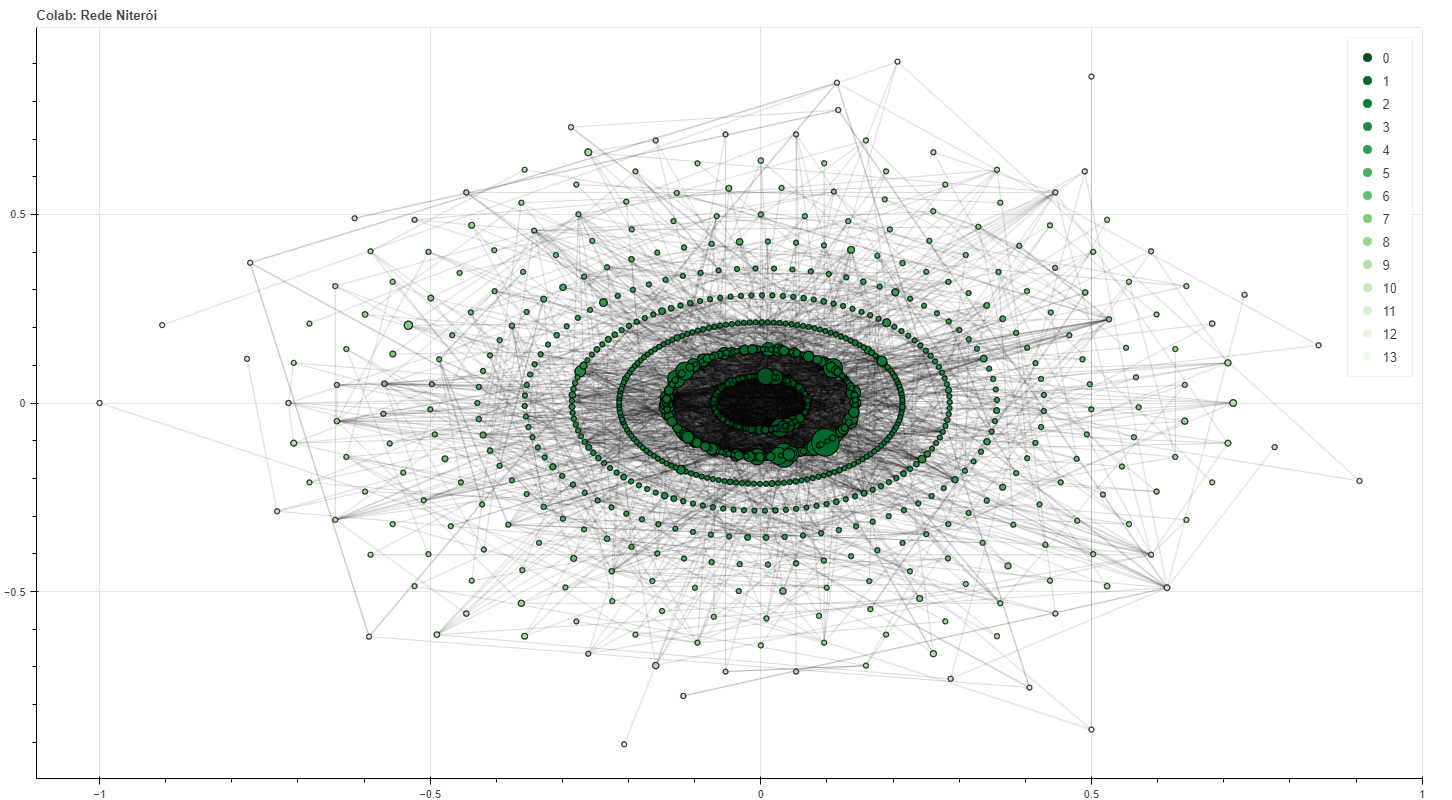
\includegraphics[scale=0.3]{images/bokeh_plot_niteroi.png}
    \caption{Visualização interativa da rede Colab na cidade de Niterói com o layout shell, exibindo as comunidades como órbitas.}
    \label{fig:bokeh_plot_niteroi}
	\fautor
\end{figure}

No contexto da nossa pesquisa sobre câmaras de eco, a escolha do algoritmo de detecção de comunidades pode influenciar significativamente nossas conclusões. Comunidades menores, como as identificadas pelo algoritmo de Louvain, podem indicar grupos mais coesos e isolados, que são características típicas de câmaras de eco. Por outro lado, comunidades maiores, como as identificadas pelo algoritmo de modularidade gananciosa, podem representar grupos mais diversificados e interconectados.

A classe \texttt{NetworkPlotter} em nossa abordagem programática é agnóstica quanto ao método de detecção de comunidades, permitindo flexibilidade na escolha do algoritmo. Isso é crucial para uma análise robusta, pois nos permite comparar e contrastar resultados de diferentes algoritmos e escolher aquele que melhor se adapta ao nosso contexto e objetivos de pesquisa.

A disposição espacial dos nós em uma visualização de rede, conhecida como layout, é crucial para a interpretação intuitiva da estrutura da rede. Diferentes estratégias de layout podem revelar diferentes aspectos da rede, desde agrupamentos locais até a estrutura global. A classe \texttt{NetworkPlotter} suporta diferentes layouts através do design pattern \textit{strategy}. O layout Kamada-Kawai, que optamos por utilizar, é uma técnica baseada em um modelo de molas. Neste modelo, os nós são tratados como partículas carregadas que se repelem mutuamente, enquanto as arestas são tratadas como molas que tentam manter os nós a uma distância desejada um do outro. O objetivo é encontrar uma disposição que minimize a energia do sistema, resultando em uma representação visual equilibrada da rede. Esta abordagem foi introduzida por \citeonline{1989_Kamada}. A escolha deste layout para nossa visualização foi motivada por sua capacidade de produzir representações claras e bem distribuídas de redes complexas, facilitando a identificação de agrupamentos e relações entre os nós.

Para facilitar a visualização e exploração da rede, o código utiliza a biblioteca Bokeh para criar um gráfico interativo. O gráfico resultante exibe os nós e suas conexões, com tamanhos e cores que refletem as métricas de interesse. Além disso, a inclusão das comunidades do grafo proporciona uma análise mais aprofundada da estrutura e organização da rede, permitindo a identificação de agrupamentos ou módulos.

Em resumo, o código implementa uma abordagem de ARS com ênfase na análise de grafos, métricas de grau e centralidade, normalização de tamanho de nós e visualização interativa. Essa combinação de técnicas e algoritmos fornece uma plataforma flexível para explorar redes sociais complexas, identificar nós de destaque e compreender a estrutura e dinâmica da rede em estudo.

Apesar das visualizações bidimensionais serem amplamente utilizadas e oferecerem insights valiosos sobre a estrutura da rede, elas têm suas limitações, especialmente quando se trata de redes de grande escala e densamente conectadas. Nestes casos, uma representação bidimensional pode não ser suficiente para capturar e representar adequadamente todas as nuances e complexidades da rede. É aqui que a visualização em três dimensões (3D) entra em cena, abrindo um novo horizonte de possibilidades para a análise e interpretação de estruturas complexas. A capacidade de explorar uma rede em 3D oferece uma perspectiva mais rica, permitindo aos pesquisadores observar agrupamentos, hierarquias e outras características estruturais de maneira mais intuitiva. Neste contexto, a biblioteca Plotly emerge como uma ferramenta poderosa, proporcionando visualizações interativas em 3D que são tanto esteticamente agradáveis quanto informativas.

O NetworkX oferece suporte nativo para layouts em 3D através da opção \texttt{dim}. Ao definir \texttt{dim=3}, os algoritmos de layout, como o Kamada-Kawai, podem ser adaptados para produzir coordenadas tridimensionais para os nós da rede. Esta flexibilidade é crucial para a transição de visualizações bidimensionais para tridimensionais.

A visualização em 3D oferece vários benefícios. Primeiramente, ela permite uma melhor distinção entre agrupamentos de nós, especialmente em redes densas. Além disso, a terceira dimensão pode ser usada para representar uma métrica adicional, como o tempo ou outro atributo nodal, proporcionando uma camada extra de informação. A classe \texttt{NetworkPlotter3D}, que desenvolvemos, aproveita essas vantagens, permitindo visualizações tridimensionais ricas e interativas de redes complexas.

\begin{figure}[h]
\centering
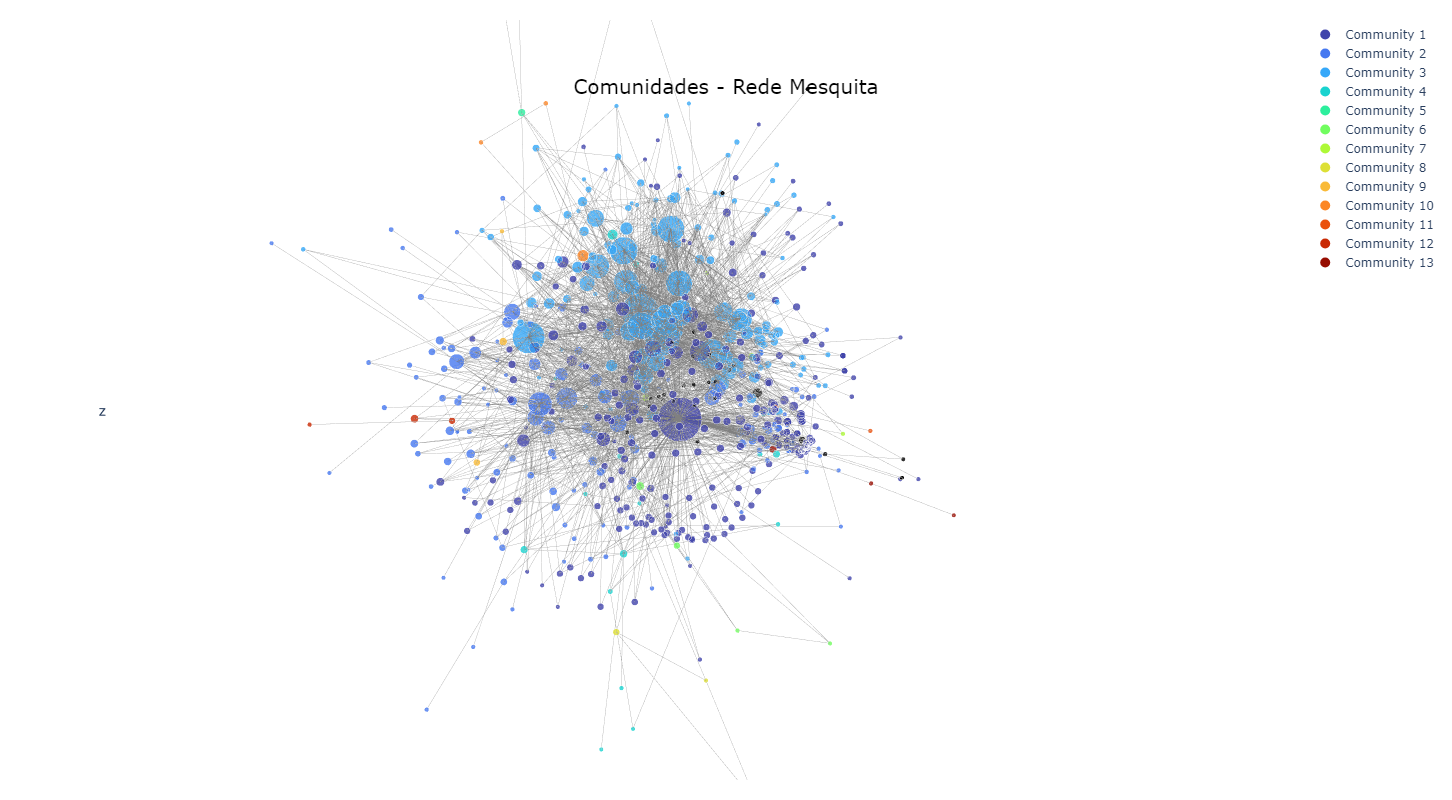
\includegraphics[scale=0.3]{images/3d_plot_example.png}
\caption{Exemplo de visualização da rede em 3D utilizando a classe \texttt{NetworkPlotter3D}. A densidade da rede pode causar o fenomeno de hairball, dificultando a interpretação.}
\label{fig:3d_plot_example}
\fautor
\end{figure}

Ao trabalhar com redes de grande escala, um obstáculo recorrente é o fenômeno denominado "hairball" (bola de pelo) \cite{2016_Tang}. Esse fenômeno manifesta-se quando a densidade de nós e arestas é tão elevada que a visualização resulta em uma aglomeração confusa, comprometendo a clareza e a interpretação. Embora o layout Kamada-Kawai apresente diversas qualidades, ele pode intensificar esse desafio em redes extensas. Isso acontece porque esse layout visa reduzir os comprimentos das arestas, o que pode ocasionar uma sobreposição indesejada de nós e arestas.

Para abordar esse desafio, introduzimos uma função de layout personalizada. Esta função utiliza heurísticas específicas para posicionar os nós de maneira que os membros da mesma comunidade sejam agrupados mais próximos, com base na influência (eigencentrality) de cada nó dentro de sua comunidade. Ao fazer isso, conseguimos uma separação clara entre diferentes comunidades, tornando-as mais notáveis e reduzindo o efeito "hairball". Esta abordagem personalizada destaca a importância de adaptar as técnicas de visualização às características específicas da rede em estudo, garantindo representações claras e informativas.

\begin{figure}[h]
	\centering
	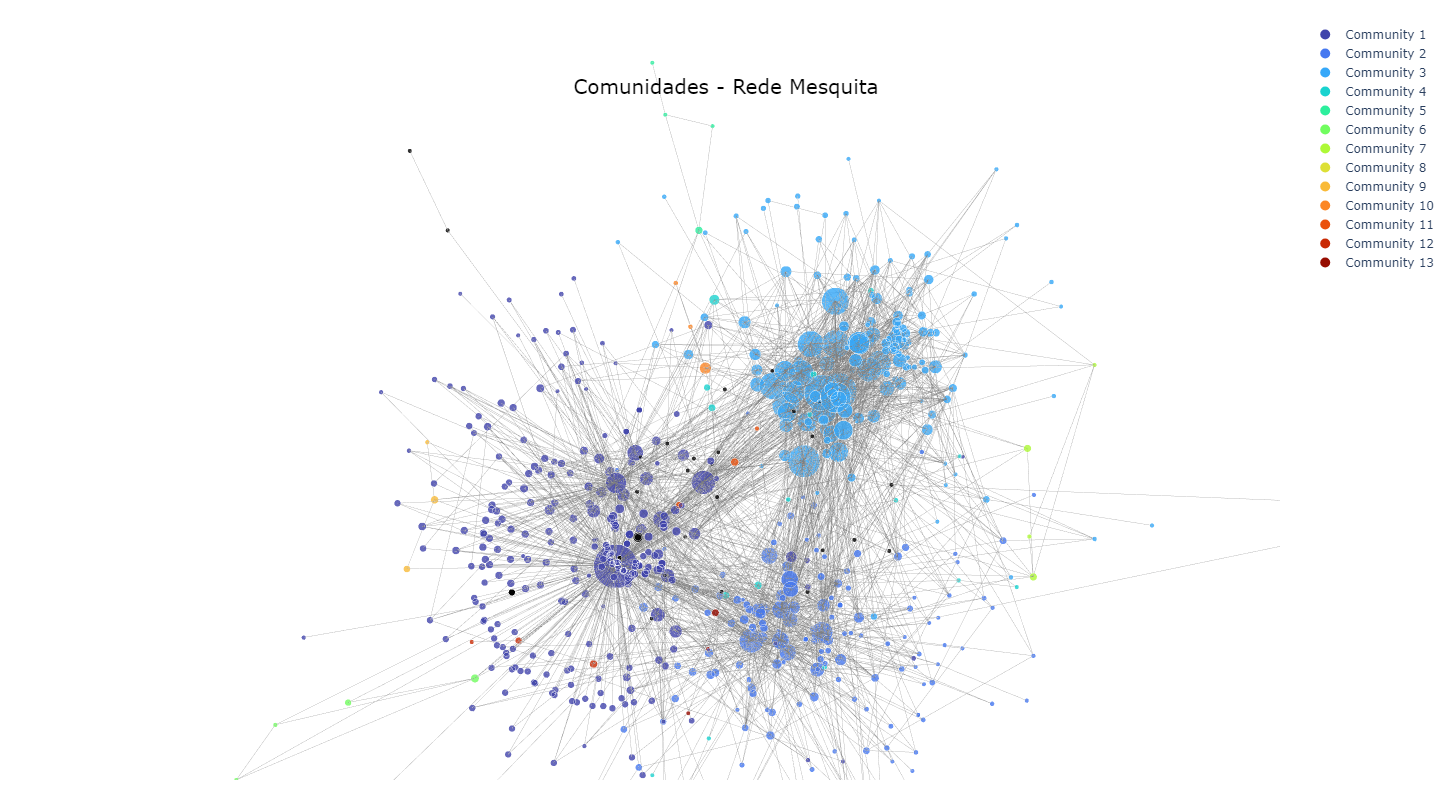
\includegraphics[scale=0.3]{images/3d_plot_hairball_buster.png}
	\caption{Exemplo de visualização da rede em 3D utilizando técnicas de layout personalizadas para reduzir o fenômeno de hairball.}
	\label{fig:3d_plot_hairball_buster}
	\fautor
\end{figure}

\section{Resultados e Discussão}

A análise exploratória de redes é uma ferramenta poderosa que nos permite desvendar as complexidades das interações sociais e compreender as dinâmicas subjacentes. Ao explorar a rede do Colab, descobrimos padrões de conexão, centralidade e comunidades que nos forneceram insights valiosos sobre o comportamento dos usuários. Esta abordagem não apenas nos permitiu visualizar a estrutura da rede, mas também identificar os usuários mais influentes e as comunidades mais ativas. Perecebe-se que o valor agregado é uma compreensão mais profunda das interações dos usuários, permitindo-nos tomar decisões informadas sobre os padrões da rede e heurísticas para detecção de câmaras de eco.

A teoria dos grafos foi nossa bússola nessa jornada exploratória. Ela forneceu o vocabulário e as técnicas necessárias e nos guiou através dos meandros da rede, ajudando-nos a identificar os caminhos mais influentes e a entender as implicações das diferentes métricas de centralidade. Através desta teoria, fomos capazes de quantificar a importância relativa dos nós e entender a estrutura global da rede. Também foi notável durante a pesquisa sobre as aplicações da teoria em análise de redes sociais, a tendência de granularizar grandes populações em subgrupos menores, permitindo uma análise mais detalhada e a identificação de padrões de interação mais sutis, tendo na rede completa uma baseline para comparação.

Nesse sentido, a topologia da rede do Colab é uma tapeçaria rica e diversificada de conexões e nós. A tabela de topologia nos oferece uma visão panorâmica da rede, permitindo-nos identificar características-chave, como a densidade da rede, o grau médio e a distribuição do grau. Estas métricas nos dão uma visão clara de como os usuários interagem e se conectam uns com os outros.

Durante nossa análise uma das primeiras observações que chamou atenção foi um alto número de cliques, que são agrupamentos de usuários altamente interconectados, indicando áreas de interação intensa e, possivelmente, a formação de comunidades centradas em tópicos específicos. Este fenômeno, característico de redes sociais dinâmicas, sugere a existência de subgrupos altamente engajados na plataforma. Paralelamente, ao avaliar as tendências de interação ao longo do tempo, conforme explorado em \autoref{sec:engajamento}, notamos um aumento nas curtidas e comentários, enquanto as conexões e avaliações de comentários apresentam uma tendência decrescente. Este padrão pode indicar uma evolução na forma como os usuários interagem, talvez focando mais em discussões em grupo do que em estabelecer novas conexões. Na teoria dos grafos, isso pode ser interpretado como uma evolução na estrutura da rede, onde os nós tendem a formar agrupamentos mais densos, potencialmente facilitando a formação de câmaras de eco. Esta observação nos sugere que, enquanto a plataforma está fomentando discussões engajadas, pode ser benéfico implementar estratégias para encorajar a formação de novas conexões, evitando assim a estagnação da rede e promovendo uma diversidade de interações. A análise de tais padrões complexos e dinâmicos é vital para entender a saúde e o crescimento sustentável da rede social, e abre avenidas para a exploração de estratégias de engajamento mais nuanceadas e eficazes.

Seguindo a estratégia de granularidade, o próximo passo foi separar a rede em comunidades, utilizamos algoritmos de detecção de comunidades, como o algoritmo de Louvain. Esses algoritmos nos permitiram identificar subgrupos dentro da rede que compartilham interesses ou características comuns, proporcionando uma visão mais granular da rede. Ao analisarmos as métricas resultantes desse processo, uma série de insights significativos emergem, contribuindo para nossa compreensão das dinâmicas das comunidades avaliadas.

Em primeiro lugar, a métrica de modularidade revelou um valor de 0.520, indicando que a divisão da rede em comunidades pelo algoritmo de Louvain é altamente significativa. Isso sugere que a estrutura da rede possui subgrupos bem definidos, onde os nós internos compartilham conexões mais densas do que com nós externos às suas respectivas comunidades. Esse nível de modularidade é fundamental para a identificação das câmaras de eco, uma vez que tais grupos tendem a ser caracterizados por uma alta coesão interna.

A distribuição dos nós por classes de modularidade é igualmente esclarecedora. Com 28\% dos nós pertencentes à Classe 1 e aproximadamente 17\% à Classe 2, percebemos que algumas comunidades são mais numerosas do que outras. Isso sugere que existem comunidades dominantes, que podem ter um papel relevante na amplificação de determinadas vozes ou crenças. Por outro lado, a presença de várias classes com menos de 1\% dos nós aponta para a existência de comunidades menores e mais especializadas, que podem desempenhar papéis igualmente importantes na disseminação de informações.

Outro insight notável provém da análise da centralidade dos usuários. Observamos que 21.04\% dos usuários têm um grau de entrada (in-degree) de 1, o que pode indicar uma forte presença de usuários periféricos na rede. Esses usuários com baixa centralidade podem ser elementos cruciais na disseminação de informações em câmaras de eco, uma vez que podem atuar como pontes entre comunidades ou grupos de interesse. Portanto, a análise de centralidade nos permite identificar não apenas os atores centrais, mas também aqueles que desempenham papéis de ligação essenciais. Com relação à centralidade de eigenvector, outra métrica crucial em nossa análise, observamos uma diversidade de valores que indicam diferentes níveis de influência dos nós na rede. Cerca de 10.23\% dos nós apresentam uma centralidade de eigenvector de 0.0, o que sugere que eles podem ter uma influência significativa na rede. Esses nós podem atuar como pontos de referência para a disseminação de informações, contribuindo para a formação de câmaras de eco. Além disso, os valores variados de centralidade de eigenvector, refletem a complexidade das interações na rede. A identificação desses nós com diferentes níveis de centralidade é fundamental para entender como a informação flui e como as câmaras de eco podem se formar e evoluir em diferentes partes da rede. Essa análise de centralidade de eigenvector complementa nossa compreensão das dinâmicas da rede, fornecendo informações adicionais sobre os atores-chave que desempenham papéis significativos na formação das câmaras de eco.

\begin{figure}[h]
    \centering
    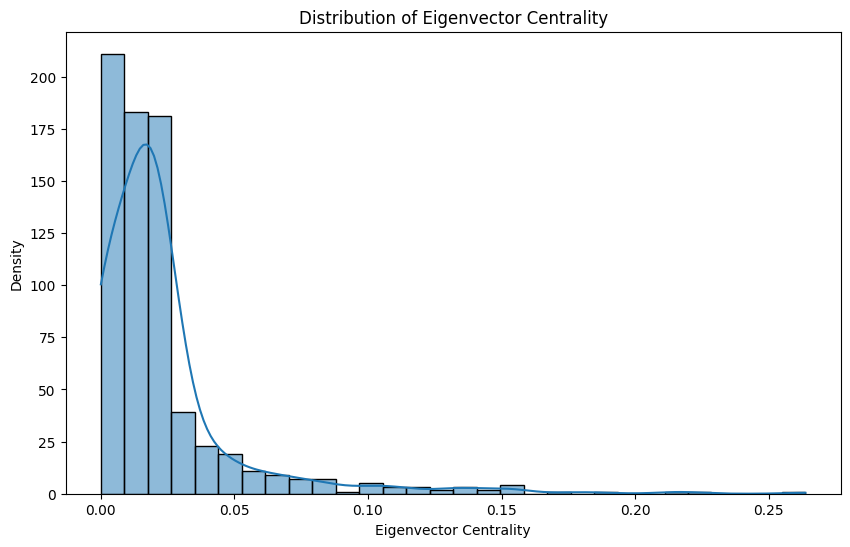
\includegraphics[scale=0.6]{images/eigencentrality.png}
    \caption{Distribuição da centralidade de eigenvector dos nós da rede.}
    \label{fig:eigencentrality}
	\fautor
\end{figure}

Analisando a demografia dos usuários, identificamos uma distribuição de gênero que favorece ligeiramente o sexo masculino, com 58.41\%, em comparação com 40.64\% de mulheres. Isso pode ter implicações na formação de câmaras de eco, uma vez que a composição demográfica influencia a dinâmica da comunicação e das crenças. Além disso, a predominância de usuários com formação de superior (54.3\%) sugere que essa rede pode estar focada em debates acadêmicos ou tópicos de maior complexidade. Essa informação é vital para entender o contexto das câmaras de eco, pois a educação desempenha um papel significativo na formação de opiniões e crenças.

A análise de idade revela uma distribuição diversificada, com nenhum grupo etário representando uma proporção dominante. Isso sugere que a rede é composta por indivíduos de diferentes faixas etárias, o que pode contribuir para a diversidade de opiniões e perspectivas. Essa heterogeneidade demográfica é relevante para a detecção de câmaras de eco, uma vez que grupos de diferentes idades podem ter abordagens distintas em relação a determinados tópicos.

A análise da excentricidade (eccentricity) da rede oferece informações sobre como os nós estão distribuídos em termos de sua distância em relação aos outros nós. Notamos que a maioria dos nós (38.25\%) possui uma excentricidade de 0, indicando que eles estão no centro da rede e, portanto, podem desempenhar papéis centrais na disseminação de informações. Por outro lado, 19.33\% dos nós têm uma excentricidade de 10, o que pode indicar a presença de nós periféricos que estão mais distantes dos demais. Essa análise da excentricidade nos permite identificar como a informação pode fluir na rede, destacando tanto os atores centrais quanto os periféricos que podem influenciar a formação de câmaras de eco.

Em resumo, a análise quantitativa dos dados resultantes da detecção de comunidades por meio do algoritmo de Louvain oferece insights cruciais para nossa compreensão das dinâmicas das câmaras de eco e das comunidades avaliadas. A modularidade da rede, a distribuição demográfica dos usuários, a centralidade dos atores e a análise de excentricidade são aspectos essenciais que nos permitem identificar padrões de interação e influência. Essas descobertas são fundamentais para entender como as câmaras de eco podem se formar e operar dentro desta rede, bem como para desenvolver estratégias eficazes de intervenção e mitigação quando necessário.

Ao focar nas três cidades com mais interações - Niterói, Santo André e Mesquita - pudemos obter uma visão mais detalhada das dinâmicas locais. Esta abordagem nos permitiu comparar e contrastar as redes destas cidades e entender as nuances regionais. A comparação da topologia das redes destas três cidades é fascinante. Mesquita, por exemplo, tem um usuário central com muitas conexões, enquanto Santo André tem vários núcleos descentralizados. Niterói, por sua vez, tem uma rede densa e integrada, indicando uma comunidade altamente interconectada. As comunidades em cada uma destas cidades também são distintas. Em Mesquita e Santo André, vemos distribuições semelhantes de comunidades, enquanto Niterói tem um cluster específico que se destaca. Estas diferenças refletem as características únicas e os padrões de interação de cada cidade.

Com as comunidades já classificadas, abre-se uma porta para a exploração mais profunda da detecção de câmaras de eco. Essas comunidades representam agrupamentos naturais de usuários em uma rede social, definidos por uma maior densidade de conexões entre seus membros. No entanto, é crucial reconhecer que nem todas as comunidades são câmaras de eco. A distinção entre esses dois conceitos é essencial para a pesquisa em questão, pois visa estabelecer critérios claros e heurísticas para a identificação precisa das câmaras de eco dentro das comunidades.

A metodologia proposta por \citeonline{2023_Atiqi_BOOK}, juntamente com a modelagem baseada em agentes, surge como uma abordagem promissora nesse contexto. Ao considerar cada usuário como um agente e simular suas interações dentro das comunidades previamente identificadas, é possível explorar como as opiniões são moldadas, reforçadas ou até mesmo silenciadas dentro desses grupos. A modelagem baseada em agentes permite analisar dinamicamente como os comportamentos individuais se traduzem em padrões coletivos de comportamento e opinião, tornando-se uma ferramenta valiosa para identificar grupos que compartilham opiniões semelhantes.

No entanto, este processo apresenta desafios significativos. Primeiramente, é preciso diferenciar comunidades normais de câmaras de eco. A simples existência de uma comunidade coesa não implica necessariamente a presença de uma câmara de eco. Portanto, a definição de critérios claros para distinguir entre esses dois conceitos é uma etapa crucial no desenvolvimento da pesquisa.

Além disso, a modelagem baseada em agentes é uma abordagem complexa, exigindo a definição cuidadosa de regras e parâmetros que governam as interações dos agentes. A dinâmica temporal das redes sociais também precisa ser considerada, uma vez que as opiniões podem evoluir ao longo do tempo, o que requer uma modelagem dinâmica.

A detecção eficaz de câmaras de eco após a identificação de comunidades requer uma análise profunda do conteúdo compartilhado e das interações entre os usuários. A análise de conteúdo pode revelar padrões de homogeneidade nas opiniões e na disseminação de informações. No \autoref{chapter:07_sentiment} abordamos a análise e a classificação do conteúdo dos usuários. Essas métricas serão usadas como insumos para as heuristicas desenvolvidas a partir da simulação de interações entre agentes, com o intuito de destacar como as opiniões podem se polarizar ou se fortalecer dentro das comunidades.

Em última análise, a combinação do técnicas eficazes de detecção de comunidades com a modelagem baseada em agentes oferece uma abordagem promissora para a identificação e compreensão das câmaras de eco em redes sociais. No entanto, é fundamental abordar os desafios mencionados e estabelecer heurísticas confiáveis para diferenciar eficazmente as câmaras de eco das comunidades tradicionais, contribuindo assim para uma compreensão mais profunda da dinâmica das redes sociais contemporâneas.

Além dos insights mencionados, é importante destacar a diversidade da rede Colab. A plataforma é um reflexo da sociedade, com usuários de diferentes idades, gêneros, etnias e níveis de educação. No entanto, observamos uma predominância de usuários masculinos, brancos e com ensino superior completo. Esta observação nos leva a refletir sobre a inclusão e representatividade na plataforma.

Olhando para o futuro, produzimos grafos no Gephi que podem ser exportados para CSV e utilizados em algoritmos em Python. Estes artefatos complementam nossa abordagem programática, permitindo-nos combinar análise visual com análise computacional.

Em conclusão, a análise da rede social do Colab nos proporcionou uma compreensão profunda das interações e dinâmicas dos usuários. Estes insights são cruciais para informar decisões estratégicas, melhorar a plataforma e promover uma comunicação mais eficaz com os cidadãos. Além disso, a metodologia desenvolvida pode ser aplicada a outras redes sociais, permitindo uma compreensão mais profunda das dinâmicas das redes sociais contemporâneas.